\chapter{歷代志上}
\section{家譜 1-9 }
%\subsection{亞當及亞伯拉罕的後裔 1 }
\subsection{亞當的後裔 1:1-27}
\subsubsection{挪亞生閃、含、雅弗 1:1-4}
亞當生塞特，塞特生以挪士， 2 以挪士生該南，該南生瑪勒列，瑪勒列生雅列， 3 雅列生以諾，以諾生瑪土撒拉，瑪土撒拉生拉麥， 4 拉麥生挪亞，挪亞生閃、含、雅弗。

\begin{forest}
  for tree={
    child anchor=west,
    parent anchor=east,
    grow=east,
    draw,
    anchor=west,
    edge path={
      \noexpand\path[\forestoption{edge}]
        (.child anchor) -| +(-5pt,0) -- +(-5pt,0) |-
        (!u.parent anchor)\forestoption{edge label};
    },
  }
  [亞當[塞特[以挪士[該南[瑪勒列[雅列[以諾[瑪土撒拉[拉麥[挪亞[閃][含][雅弗]]]]]]]]]]]
  ]
\end{forest}

\subsubsection{雅弗 1:5-7}
\begin{figure}[H]
\begin{minipage}{0.5\textwidth}
\begin{forest}
  for tree={
    child anchor=west,
    parent anchor=east,
    grow=east,
    draw,
    anchor=west,
    edge path={
      \noexpand\path[\forestoption{edge}]
        (.child anchor) -| +(-5pt,0) -- +(-5pt,0) |-
        (!u.parent anchor)\forestoption{edge label};
    },
  }
  [雅弗[歌篾[亞實基拿][利法][陀迦瑪]]
    	  [瑪各][瑪代]
    		[雅完[以利沙][他施][基提][多單]]
    		[土巴][米設][提拉] ]
  ]
\end{forest}
\end{minipage}
%\hfill
\begin{minipage}{0.3\textwidth}
雅弗的兒子是歌篾、瑪各、瑪代、雅完、土巴、米設、提拉。 6 歌篾的兒子是亞實基拿、低法(《創》10:3作「利法」)、陀迦瑪。 7 雅完的兒子是以利沙、他施、基提、多單(有作「羅單」的)。 
\end{minipage}
\end{figure}

\subsubsection{含 1:8-16}
\begin{figure}[H]
\begin{minipage}{0.725\textwidth}
\begin{forest}
  for tree={
    child anchor=west,
    parent anchor=east,
    grow=east,
    draw,
    anchor=west,
    edge path={
      \noexpand\path[\forestoption{edge}]
        (.child anchor) -| +(-5pt,0) -- +(-5pt,0) |-
        (!u.parent anchor)\forestoption{edge label};
    },
  }
  [含[古實[哈腓拉][撒弗他][西巴]
    			[拉瑪[示巴][底但][寧錄（英勇的獵戶）[示拿地[巴別][以力][亞甲][甲尼]]
    															 [亞述[尼尼微][利河伯][迦拉][利鮮]]]]
    			[撒弗提迦]]
    			[麥西[路低人][亞拿米人][利哈比人][拿弗土希人]
    				  [帕斯魯細人][迦斯路希人][迦斐託人[非利士人]]]
    			[弗]
    			[迦南[西頓][赫][耶布斯人][亞摩利人][革迦撒人][希未人]
    			     [亞基人][西尼人][亞瓦底人][洗瑪利人][哈馬人]]
	]
  ]
\end{forest}
\end{minipage}
%\hfill
\begin{minipage}{0.2\textwidth}
8 含的兒子是古實、麥西、弗、迦南。 9 古實的兒子是西巴、哈腓拉、撒弗他、拉瑪、撒弗提迦。拉瑪的兒子是示巴、底但。 10 古實生寧錄，他為世上英雄之首。 11 麥西生路低人、亞拿米人、利哈比人、拿弗土希人、 12 帕斯魯細人、迦斯路希人、迦斐托人，從迦斐托出來的有非利士人。 13 迦南生長子西頓，又生赫， 14 和耶布斯人、亞摩利人、革迦撒人、 15 希未人、亞基人、西尼人、 16 亞瓦底人、洗瑪利人並哈馬人。
\end{minipage}
\end{figure}



\subsubsection{ 閃 1:17-27}
\newpage
\begin{figure}[H]
\begin{minipage}{0.725\textwidth}
%\hfill
\vspace{-5mm}
\begin{forest}
  for tree={
    child anchor=west,
    parent anchor=east,
    grow=east,
    draw,
    anchor=west,
    edge path={
      \noexpand\path[\forestoption{edge}]
        (.child anchor) -| +(-5pt,0) -- +(-5pt,0) |-
        (!u.parent anchor)\forestoption{edge label};
    },
  }
  [閃
    	[以攔][亞述][路德]
    	[亞法撒[沙拉[希伯[法勒(分),tikz={\node [draw, red,fit=()(!1)(!ll)(!lll)(!llll)(!lllll)]{};}[拉吳[西鹿[拿鶴[他拉[亞伯蘭]]]]]]
    	                 [約坍[亞摩答][沙列][哈薩瑪非][耶拉]
    								  [哈多蘭][烏薩][德拉][俄巴路][亞比瑪利]
    								  [示巴][阿斐][哈腓拉][約巴]]]]]
    	[亞蘭[烏斯][戶勒][基帖][瑪施]]
    ]
  ]
\end{forest}
\end{minipage}
%\hfill
\begin{minipage}{0.25\textwidth}
17 閃的兒子是以攔、亞述、亞法撒、路德、亞蘭、烏斯、戶勒、基帖、米設(《創》10:23作「瑪施」)。 18 亞法撒生沙拉，沙拉生希伯。 19 希伯生了兩個兒子，一個名叫法勒(分)，因為那時人就分地居住；法勒的兄弟名叫約坍。 20 約坍生亞摩答、沙列、哈薩瑪非、耶拉、 21 哈多蘭、烏薩、德拉、 22 以巴錄、亞比瑪利、示巴、 23 阿斐、哈腓拉、約巴，這都是約坍的兒子。24 閃生亞法撒，亞法撒生沙拉， 25 沙拉生希伯，希伯生法勒，法勒生拉吳， 26 拉吳生西鹿，西鹿生拿鶴，拿鶴生他拉， 27 他拉生亞伯蘭，亞伯蘭就是亞伯拉罕。
\end{minipage}
\end{figure}



\subsection{亞伯拉罕的後裔 1:28-34}
%\hfill \break
%\hfill \break
\begin{figure}[H]
\vspace{-5mm}
\begin{minipage}{0.5\textwidth}
\begin{forest}
  for tree={
    child anchor=west,
    parent anchor=east,
    grow=east,
    draw,
    anchor=west,
    edge path={
      \noexpand\path[\forestoption{edge}]
        (.child anchor) -| +(-5pt,0) -- +(-5pt,0) |-
        (!u.parent anchor)\forestoption{edge label};
    },
  }
  [亞伯拉罕[以撒]
    	     [以實瑪利[尼拜約][基達][押德別][米比衫]
    	              [度瑪][瑪撒][哈達][提瑪][伊突][拿非施][基底瑪]]
    	     [心蘭]
      	  [約珊[示巴][底但]]
      	  [米但]
      	  [米甸[以法][以弗][哈諾][亞比大][以勒大]]      	  
      	  [伊施巴] 
      	  [書亞]        	          	       	        	       	           	  
  ]
\end{forest}
\end{minipage}
%\hfill
\begin{minipage}{0.25\textwidth}
亞伯拉罕的兒子是以撒、以實瑪利。 29 以實瑪利的兒子記在下面：以實瑪利的長子是尼拜約，其次是基達、亞德別、米比衫、 30 米施瑪、度瑪、瑪撒、哈達、提瑪、 31 伊突、拿非施、基底瑪。這都是以實瑪利的兒子。32 亞伯拉罕的妾基土拉所生的兒子就是心蘭、約珊、米但、米甸、伊施巴、書亞。約珊的兒子是示巴、底但。 33 米甸的兒子是以法、以弗、哈諾、亞比大、以勒大。這都是基土拉的子孫。34 亞伯拉罕生以撒，以撒的兒子是以掃和以色列。
\end{minipage}
\end{figure}

%\newpage
\subsection{以掃的後裔 1:35-54}
\subsubsection{以掃的後裔 1:35-37}
\begin{figure}[H]
\vspace{-5mm}
\begin{minipage}{0.5\textwidth}
\begin{forest}
  for tree={
    child anchor=west,
    parent anchor=east,
    grow=east,
    draw,
    anchor=west,
    edge path={
      \noexpand\path[\forestoption{edge}]
        (.child anchor) -| +(-5pt,0) -- +(-5pt,0) |-
        (!u.parent anchor)\forestoption{edge label};
    },
  }
  [以撒[以掃(以東）[以利法[提幔][阿抹][洗玻][迦坦][基納斯][亭納][亞瑪力]]
  				[流珥[拿哈][謝拉][沙瑪][米撒]]
  				[雅蘭][可拉][耶烏施]]
       [以色列]    	          	       	        	       	           	  
  ]
\end{forest}
\end{minipage}
%\hfill
\begin{minipage}{0.25\textwidth}
以掃的兒子是以利法、流珥、耶烏施、雅蘭、可拉。 36 以利法的兒子是提幔、阿抹、洗玻、迦坦、基納斯、亭納、亞瑪力。 37 流珥的兒子是拿哈、謝拉、沙瑪、米撒。
\end{minipage}
\end{figure}

\subsubsection{西珥之後裔 1:38-42}
\begin{figure}[H]
\vspace{-5mm}
\begin{minipage}{0.5\textwidth}
\begin{forest}
  for tree={
    child anchor=west,
    parent anchor=east,
    grow=east,
    draw,
    anchor=west,
    edge path={
      \noexpand\path[\forestoption{edge}]
        (.child anchor) -| +(-5pt,0) -- +(-5pt,0) |-
        (!u.parent anchor)\forestoption{edge label};
    },
  }
  [西珥[羅坍[何利][荷幔]]
       [亭納(羅坍的妹妹)]
  		 [朔巴[亞勒文][瑪拿轄][以巴錄][示非][阿南]]
       [祭便[亞雅][亞拿]]
       [亞拿[底順]]
       [底順[哈默蘭][伊是班][益蘭][基蘭]]
       [以察[辟罕][撒番][亞干]]                         	          	       	        	    [底珊[烏斯][亞蘭]]	  
  ]
\end{forest}
 \end{minipage}
%\hfill
\begin{minipage}{0.25\textwidth}
西珥的兒子是羅坍、朔巴、祭便、亞拿、底順、以察、底珊。 39 羅坍的兒子是何利、荷幔，羅坍的妹子是亭納。 40 朔巴的兒子是亞勒文、瑪拿轄、以巴錄、示非、阿南。祭便的兒子是亞雅、亞拿。 41 亞拿的兒子是底順。底順的兒子是哈默蘭、伊是班、益蘭、基蘭。 42 以察的兒子是辟罕、撒番、亞干。底珊的兒子是烏斯、亞蘭。
\end{minipage}
\end{figure}    

           
\subsubsection{以東諸王 1:43-50}
以色列人未有君王治理之先，在以東地做王的記在下面。有比珥的兒子比拉，他的京城名叫亭哈巴。 44 比拉死了，波斯拉人謝拉的兒子約巴接續他做王。 45 約巴死了，提幔地的人戶珊接續他做王。 46 戶珊死了，比達的兒子哈達接續他做王，這哈達就是在摩押地殺敗米甸人的，他的京城名叫亞未得。 47 哈達死了，瑪士利加人桑拉接續他做王。 48 桑拉死了，大河邊的利河伯人掃羅接續他做王。 49 掃羅死了，亞革波的兒子巴勒哈南接續他做王。 50 巴勒哈南死了，哈達接續他做王，他的京城名叫巴伊，他的妻子名叫米希她別，是米薩合的孫女、瑪特列的女兒。

\subsubsection{以東諸族長 1:51-54}
哈達死了，以東人的族長有亭納族長、亞勒瓦族長、耶帖族長、 52 阿何利巴瑪族長、以拉族長、比嫩族長、 53 基納斯族長、提幔族長、米比薩族長、 54 瑪基疊族長、以蘭族長。這都是以東人的族長。

\subsection{以色列之後裔 2:1-2}
以色列的兒子是魯本、西緬、利未、猶大、以薩迦、西布倫、 2 但、約瑟、便雅憫、拿弗他利、迦得、亞設。

\subsection{猶大的後裔 2-4:20 }
\subsubsection{猶大之後裔 2:3-8}
猶大的兒子是珥、俄南、示拉，這三人是迦南人書亞女兒所生的。猶大的長子珥在耶和華眼中看為惡，耶和華就使他死了。 4 猶大的兒婦她瑪給猶大生法勒斯和謝拉。猶大共有五個兒子。

5 法勒斯的兒子是希斯崙、哈母勒。 6 謝拉的兒子是心利、以探、希幔、甲各、大拉(達大)，共五人。 7 迦米的兒子是亞干，這亞干在當滅的物上犯了罪，連累了以色列人。 8 以探的兒子是亞撒利雅。


\subsubsection{希斯崙之後裔 2:9-17}
希斯崙所生的兒子是耶拉篾、蘭、基路拜。 10 蘭生亞米拿達，亞米拿達生拿順，拿順做猶大人的首領。 11 拿順生撒門，撒門生波阿斯， 12 波阿斯生俄備得，俄備得生耶西。 13 耶西生長子以利押，次子亞比拿達，三子示米亞(沙瑪，《撒上》16:9)， 14 四子拿坦業，五子拉代， 15 六子阿鮮，七子大衛， 16 他們的姐妹是洗魯雅和亞比該。洗魯雅的兒子是亞比篩、約押、亞撒黑，共三人。 17 亞比該生亞瑪撒，亞瑪撒的父親是以實瑪利人益帖。

\subsubsection{迦勒之後裔 2:18-55}
希斯崙的兒子迦勒娶阿蘇巴和耶略為妻，阿蘇巴的兒子是耶設、朔罷、押墩。 19 阿蘇巴死了，迦勒又娶以法她，生了戶珥。 20 戶珥生烏利，烏利生比撒列。

21 希斯崙正六十歲娶了基列父親瑪吉的女兒，與她同房，瑪吉的女兒生了西割。 22 西割生睚珥，睚珥在基列地有二十三個城邑。 23 （後來基述人和亞蘭人奪了睚珥的城邑，並基納和其鄉村，共六十個。）這都是基列父親瑪吉之子的。 24 希斯崙在迦勒以法他死後，他的妻亞比雅給他生了亞施戶，亞施戶是提哥亞的父親。

25 希斯崙的長子耶拉篾生長子蘭，又生布拿、阿連、阿鮮、亞希雅。 26 耶拉篾又娶一妻，名叫亞她拉，是阿南的母親。 27 耶拉篾長子蘭的兒子是瑪斯、雅憫、以結。 28 阿南的兒子是沙買、雅大。沙買的兒子是拿答、亞比述。 29 亞比述的妻名叫亞比孩，亞比孩給他生了亞辦和摩利。 30 拿答的兒子是西列、亞遍。西列死了，沒有兒子。 31 亞遍的兒子是以示，以示的兒子是示珊，示珊的兒子是亞來。 32 沙買兄弟雅大的兒子是益帖、約拿單。益帖死了，沒有兒子。 33 約拿單的兒子是比勒、撒薩。這都是耶拉篾的子孫。 34 示珊沒有兒子，只有女兒。示珊有一個僕人名叫耶哈，是埃及人。 35 示珊將女兒給了僕人耶哈為妻，給他生了亞太。 36 亞太生拿單，拿單生撒拔， 37 撒拔生以弗拉，以弗拉生俄備得， 38 俄備得生耶戶，耶戶生亞撒利雅， 39 亞撒利雅生希利斯，希利斯生以利亞薩， 40 以利亞薩生西斯買，西斯買生沙龍， 41 沙龍生耶加米雅，耶加米雅生以利沙瑪。

42 耶拉篾兄弟迦勒的長子米沙，是西弗之祖瑪利沙的兒子，是希伯崙之祖。 43 希伯崙的兒子是可拉、他普亞、利肯、示瑪。 44 示瑪生拉含，是約干之祖。利肯生沙買。 45 沙買的兒子是瑪雲，瑪雲是伯夙之祖。 46 迦勒的妾以法生哈蘭、摩撒、迦謝，哈蘭生迦卸。 47 雅代的兒子是利健、約坦、基珊、毗力、以法、沙亞弗。 48 迦勒的妾瑪迦生示別、特哈拿， 49 又生麥瑪拿之祖沙亞弗、抹比拿和基比亞之祖示法。迦勒的女兒是押撒。

50 迦勒的子孫，就是以法她的長子戶珥的兒子，記在下面：基列耶琳之祖朔巴， 51 伯利恆之祖薩瑪，伯迦得之祖哈勒。 52 基列耶琳之祖朔巴的子孫是哈羅以和一半米努哈人(瑪拿哈人)。 53 基列耶琳的諸族是以帖人、布特人、舒瑪人、密來人，又從這些族中生出瑣拉人和以實陶人來。 54 薩瑪的子孫是伯利恆人、尼陀法人、亞他綠伯約押人、一半瑪拿哈人、瑣利人， 55 和住雅比斯眾文士家的特拉人、示米押人、蘇甲人。這都是基尼人利甲家之祖哈末所生的。


\begin{forest}
  for tree={
    child anchor=west,
    parent anchor=east,
    grow=east,
    draw,
    anchor=west,
    edge path={
      \noexpand\path[\forestoption{edge}]
        (.child anchor) -| +(-5pt,0) -- +(-4pt,0) |-
        (!u.parent anchor)\forestoption{edge label};
    },
  }
  [以色列[流便]
         [猶大[珥]
       		   [俄南]
       		   [示拉]
       		   [法勒斯[希斯崙[耶拉篾[蘭[瑪斯][雅憫][以結]]
       		                        [布拿][阿連][亞希雅][阿鮮]
       		                        [阿南[沙買[拿答[西列][亞遍[以示[示珊[亞來][\textbf 耶哈]]]]]
       		                                  [亞比述[亞辦][摩利]]]
       		                             [雅大[益帖][約拿單[比勒][撒薩]]]]]
       		                 [蘭[亞米拿達[拿順[撒門[波阿斯[俄備得[耶西]]]]]]]
       		                 [基路拜]
       		                 [迦勒[耶設][朔罷][押墩][戶珥[烏利[比撒列]]]
       		                      [亞施戶[提哥亞]]]             		                 
       		                 [西割(基列父親瑪吉的女兒所生)[\textbf 睚珥]]]
                      [哈母勒]]
              [謝拉[心利(迦米)[\textbf 亞干]]
                   [以探[亞撒利雅]][希幔][甲各][大拉（達大）]]]         
        [但][約瑟][迦得]	
	    [亞設]	
	    [西緬]
  		   [利未]
        [以薩迦]                       	          	       	    
       [西布倫] 	   
	    [便雅憫]
	    [拿弗他利]			    	       	             
  ]
\end{forest}

\begin{forest}
  for tree={
    child anchor=west,
    parent anchor=east,
    grow=east,
    draw,
    anchor=west,
    edge path={
      \noexpand\path[\forestoption{edge}]
        (.child anchor) -| +(-3pt,0) -- +(-4pt,0) |-
        (!u.parent anchor)\forestoption{edge label};
    },
  }
  [耶哈[亞太[拿單[撒拔[以弗拉[俄備得[耶戶[亞撒利雅[希利斯]]]]]]]]
  ]       
\end{forest}
 \hfill \break
 
\begin{forest}
  for tree={
    child anchor=west,
    parent anchor=east,
    grow=east,
    draw,
    anchor=west,
    edge path={
      \noexpand\path[\forestoption{edge}]
        (.child anchor) -| +(-3pt,0) -- +(-5pt,0) |-
        (!u.parent anchor)\forestoption{edge label};
    },
  }
  [希利斯[以利亞薩[西斯買[沙龍[耶加米雅[以利沙瑪]]]]]
  ] % \hfill \break   
\end{forest}

%\newline
 %\hfill \break
 


\begin{forest}
  for tree={
    child anchor=west,
    parent anchor=east,
    grow=east,
    draw,
    anchor=west,
    edge path={
      \noexpand\path[\forestoption{edge}]
        (.child anchor) -| +(-5pt,0) -- +(-5pt,0) |-
        (!u.parent anchor)\forestoption{edge label};
    },
  }
  [迦勒[瑪迦[示別][特哈拿]]      
       [米沙[希伯崙[可拉]
       				  [他普亞]
       				  [利肯[沙買[瑪雲]]]
       				  [示瑪[拉含]]]] 
      [哈蘭[迦卸]]
      [摩撒]
      [迦謝] 
      [示別][特哈拿][沙亞弗][示法] [押撒(女兒)]   				                           		[戶珥[基列耶琳之祖朔巴[密來人[瑣拉人][以實陶人]][舒瑪人][布特人][以帖人][哈羅以和一半米努哈人]][伯利恆之祖薩瑪[基尼人利甲家之祖[蘇甲人(住雅比斯眾文士家)][示米押人(住雅比斯眾文士家)][特拉人(住雅比斯眾文士家)]][伯利恆人][尼陀法人][亞他綠伯約押人][瑣利人][一半瑪拿哈人]][伯迦得之祖哈勒]]           	       	             
  ]
\end{forest}

\begin{forest}
  for tree={
    child anchor=west,
    parent anchor=east,
    grow=east,
    draw,
    anchor=west,
    edge path={
      \noexpand\path[\forestoption{edge}]
        (.child anchor) -| +(-5pt,0) -- +(-5pt,0) |-
        (!u.parent anchor)\forestoption{edge label};
    },
  }
  [猶大[示拉[利迦之祖珥][瑪利沙之祖拉大][屬亞實比族織細麻布的各家]
  				[約敬][哥西巴人][約阿施]
  				 [薩拉(在摩押地掌權)]
  				 [雅叔比利恆]
		]
  ]
\end{forest}


\hfill \break
\begin{forest}
  for tree={
    child anchor=west,
    parent anchor=east,
    grow=east,
    draw,
    anchor=west,
    edge path={
      \noexpand\path[\forestoption{edge}]
        (.child anchor) -| +(-5pt,0) -- +(-5pt,0) |-
        (!u.parent anchor)\forestoption{edge label};
    },
  }
  [耶西[大衛] \textbf{} [亞比拿達]  [示米亞(沙瑪)]  [拿坦業]  [拉代]
       [阿鮮][以利押][洗魯雅(女）[亞比篩][約押][亞撒黑]] 
      [亞比該(女）[亞瑪撒(父親是以實瑪利人益帖)]]	       	             
  ]
\end{forest}

\subsection{大衛之諸子 3:1-9}
\begin{figure}[H]
\vspace{0mm}
\begin{minipage}{0.5\textwidth}
\begin{forest}
  for tree={
    child anchor=west,
    parent anchor=east,
    grow=east,
    draw,
    anchor=west,
    edge path={
      \noexpand\path[\forestoption{edge}]
        (.child anchor) -| +(-5pt,0) -- +(-5pt,0) |-
        (!u.parent anchor)\forestoption{edge label};
    },
  }
  [大衛[以利法列][以利雅大][以利沙瑪][雅非亞][尼斐]
  				[挪迦][以利法列][以利沙瑪][益轄]
  				[示米亞(亞米利的女兒拔書亞)]
  				[朔罷(亞米利的女兒拔書亞)]
  				[拿單(亞米利的女兒拔書亞)]
  				[所羅門(亞米利的女兒拔書亞)]
  				[以特念(以格拉生)]
  				[示法提雅(亞比他)]
  				[亞多尼雅(哈及)]
  				[押沙龍(基述王達買的女兒瑪迦)]
  				[他瑪(基述王達買的女兒瑪迦)]
  				[但以利(迦密人亞比該)]
  				[暗嫩(耶斯列人亞希暖)]                   	             
  ]
\end{forest}
\end{minipage}
%\hfill
\begin{minipage}{0.25\textwidth}
大衛在希伯崙所生的兒子記在下面：長子暗嫩，是耶斯列人亞希暖生的；次子但以利，是迦密人亞比該生的； 2 三子押沙龍，是基述王達買的女兒瑪迦生的；四子亞多尼雅，是哈及生的； 3 五子示法提雅，是亞比她生的；六子以特念，是大衛的妻以格拉生的。 4 這六人都是大衛在希伯崙生的。大衛在希伯崙做王七年零六個月，在耶路撒冷做王三十三年。 5 大衛在耶路撒冷所生的兒子是：示米亞、朔罷、拿單、所羅門，這四人是亞米利的女兒拔書亞生的； 6 還有益轄、以利沙瑪、以利法列、 7 挪迦、尼斐、雅非亞、 8 以利沙瑪、以利雅大、以利法列，共九人。 9 這都是大衛的兒子，還有他們的妹子她瑪；妃嬪的兒子不在其內。
\end{minipage}
\end{figure}  



\subsection{所羅門之後裔 3:1-9}
\hfill \break
\hfill \break
\begin{forest}
  for tree={
    child anchor=west,
    parent anchor=east,
    grow=east,
    draw,
    anchor=west,
    edge path={
      \noexpand\path[\forestoption{edge}]
        (.child anchor) -| +(-5pt,0) -- +(-5pt,0) |-
        (!u.parent anchor)\forestoption{edge label};
    },
  }
  [所羅門[羅波安[亞比雅[亞撒[約沙法[約蘭[亞哈謝[約阿施[亞瑪謝]]]]]]]]]	       	             
  ]
\end{forest}
\hfill \break
\begin{forest}
  for tree={
    child anchor=west,
    parent anchor=east,
    grow=east,
    draw,
    anchor=west,
    edge path={
      \noexpand\path[\forestoption{edge}]
        (.child anchor) -| +(-5pt,0) -- +(-5pt,0) |-
        (!u.parent anchor)\forestoption{edge label};
    },
  }
  [亞瑪謝[亞撒利雅[約坦[亞撒[亞哈斯[希西家[瑪拿西[亞們[約西亞[沙龍][西底家][約雅敬[耶哥尼雅][西底家]][約哈難]]]]]]]]]]	       	             
  ]
\end{forest}

\begin{forest}
  for tree={
    child anchor=west,
    parent anchor=east,
    grow=east,
    draw,
    anchor=west,
    edge path={
      \noexpand\path[\forestoption{edge}]
        (.child anchor) -| +(-5pt,0) -- +(-5pt,0) |-
        (!u.parent anchor)\forestoption{edge label};
    },
  }
  [耶哥尼雅[撒拉鐵][瑪基蘭]
  			  [毗大雅[所羅巴伯[米書蘭[哈舒巴][阿黑][比利家][哈撒底][于沙希悉]]
  			  						 [哈拿尼雅[毗拉提][耶篩亞][利法雅的眾子][亞珥難的眾子][俄巴底亞的眾子][示迦尼的眾子[示瑪雅[沙法][尼利雅[亞斯利干][希西家]
  			  						 [以利約乃[何大雅][以利亞實][毗萊雅][阿谷][約哈難][第萊雅][阿拿尼]]][巴利亞][以甲][哈突]]]]
  			  						 [示羅密(妹子)]]
						[示每]]
  			  [示拿薩][耶加米][何沙瑪][尼大比雅]		       	             
  ]
\end{forest}
所羅門的兒子是羅波安，羅波安的兒子是亞比雅，亞比雅的兒子是亞撒，亞撒的兒子是約沙法， 11 約沙法的兒子是約蘭，約蘭的兒子是亞哈謝，亞哈謝的兒子是約阿施， 12 約阿施的兒子是亞瑪謝，亞瑪謝的兒子是亞撒利雅，亞撒利雅的兒子是約坦， 13 約坦的兒子是亞哈斯，亞哈斯的兒子是希西家，希西家的兒子是瑪拿西， 14 瑪拿西的兒子是亞們，亞們的兒子是約西亞。 15 約西亞的長子是約哈難，次子是約雅敬，三子是西底家，四子是沙龍。 16 約雅敬的兒子是耶哥尼雅和西底家。 17 耶哥尼雅被擄，他的兒子是撒拉鐵、 18 瑪基蘭、毗大雅、示拿薩、耶加米、何沙瑪、尼大比雅。 19 毗大雅的兒子是所羅巴伯、示每。所羅巴伯的兒子是米書蘭、哈拿尼雅，他們的妹子名叫示羅密。 20 米書蘭的兒子是哈舒巴、阿黑、比利家、哈撒底、于沙希悉，共五人。 21 哈拿尼雅的兒子是毗拉提、耶篩亞，還有利法雅的眾子、亞珥難的眾子、俄巴底亞的眾子、示迦尼的眾子。 22 示迦尼的兒子是示瑪雅，示瑪雅的兒子是哈突、以甲、巴利亞、尼利雅、沙法，共六人。 23 尼利雅的兒子是以利約乃、希西家、亞斯利干，共三人。 24 以利約乃的兒子是何大雅、以利亞實、毗萊雅、阿谷、約哈難、第萊雅、阿拿尼，共七人。


\subsection{復記猶大之後裔 4:1-23}
猶大的兒子是法勒斯、希斯崙、迦米、戶珥、朔巴。 2 朔巴的兒子利亞雅生雅哈，雅哈生亞戶買和拉哈，這是瑣拉人的諸族。 3 以坦之祖的兒子是耶斯列、伊施瑪、伊得巴，他們的妹子名叫哈悉勒玻尼； 4 基多之祖是毗努伊勒；戶沙之祖是以謝珥。這都是伯利恆之祖以法她的長子戶珥所生的。 5 提哥亞之祖亞施戶有兩個妻子，一名希拉，一名拿拉。 6 拿拉給亞施戶生亞戶撒、希弗、提米尼、哈轄斯他利，這都是拿拉的兒子。 7 希拉的兒子是洗列、瑣轄、伊提南。 8 哥斯生亞諾、瑣比巴並哈崙兒子亞哈黑的諸族。 9 雅比斯比他眾弟兄更尊貴，他母親給他起名叫雅比斯，意思說：「我生他甚是痛苦。」 10 雅比斯求告以色列的神說：「甚願你賜福於我，擴張我的境界，常與我同在，保佑我不遭患難，不受艱苦。」神就應允他所求的。 11 書哈的弟兄基綠生米黑，米黑是伊施屯之祖。 12 伊施屯生伯拉巴、巴西亞並珥拿轄之祖提欣拿，這都是利迦人。 13 基納斯的兒子是俄陀聶、西萊雅。俄陀聶的兒子是哈塔； 14 憫挪太生俄弗拉。西萊雅生革夏納欣人之祖約押，他們都是匠人。 15 耶孚尼的兒子是迦勒，迦勒的兒子是以路、以拉、拿安，以拉的兒子是基納斯。 16 耶哈利勒的兒子是西弗、西法、提利、亞撒列。 17  18 以斯拉的兒子是益帖、米列、以弗、雅倫。米列娶法老女兒比提雅為妻，生米利暗、沙買和以實提摩之祖益巴。米列又娶猶大女子為妻，生基多之祖雅列、梭哥之祖希伯和撒挪亞之祖耶古鐵。 19 荷第雅的妻是拿含的妹子，她所生的兒子是迦米人基伊拉和瑪迦人以實提摩之祖。 20 示門的兒子是暗嫩、林拿、便哈南、提倫。以示的兒子是梭黑與便梭黑。 21 猶大的兒子是示拉，示拉的兒子是利迦之祖珥、瑪利沙之祖拉大和屬亞實比族織細麻布的各家， 22 還有約敬、哥西巴人、約阿施、薩拉，就是在摩押地掌權的，又有雅叔比利恆，這都是古時所記載的。 23 這些人都是窯匠，是尼他應和基低拉的居民，與王同處，為王做工。

\subsection{西緬的後裔 4:24-43}
\begin{figure}[H]
\vspace{0mm}
\begin{minipage}{0.5\textwidth}
\begin{forest}
  for tree={
    child anchor=west,
    parent anchor=east,
    grow=east,
    draw,
    anchor=west,
    edge path={
      \noexpand\path[\forestoption{edge}]
        (.child anchor) -| +(-5pt,0) -- +(-5pt,0) |-
        (!u.parent anchor)\forestoption{edge label};
    },
  }
  [西緬[尼母利][雅憫][雅立][謝拉][掃羅[沙龍[米比衫[米施瑪[哈母利[撒刻[示每(十六個兒子，六個女兒)]]]]]]]	  
  ]
\end{forest}
\end{minipage}
\vspace{-5mm}
\hspace{-60mm}
\begin{minipage}{0.8\textwidth}
西緬的兒子是尼母利、雅憫、雅立、謝拉、掃羅。 25 掃羅的兒子是沙龍，沙龍的兒子是米比衫，米比衫的兒子是米施瑪， 26 米施瑪的兒子是哈母利，哈母利的兒子是撒刻，撒刻的兒子是示每。 27 示每有十六個兒子、六個女兒，他弟兄的兒女不多，他們各家不如猶大族的人丁增多。
\end{minipage}
\end{figure}  


28 西緬人住在別是巴、摩拉大、哈薩書亞、 29 辟拉、以森、陀臘、 30 彼土利、何珥瑪、洗革拉、 31 伯瑪加博、哈薩蘇撒、伯比利、沙拉音，這些城邑直到大衛做王的時候都是屬西緬人的。 32 他們的五個城邑是以坦、亞因、臨門、陀健、亞珊， 33 還有屬城的鄉村，直到巴力。這是他們的住處，他們都有家譜。 34 還有米所巴、雅米勒、亞瑪謝的兒子約沙、 35 約珥、約示比的兒子耶戶，約示比是西萊雅的兒子，西萊雅是亞薛的兒子。 36 還有以利約乃、雅哥巴、約朔海、亞帥雅、亞底業、耶西篾、比拿雅、 37 示非的兒子細撒，示非是亞龍的兒子，亞龍是耶大雅的兒子，耶大雅是申利的兒子，申利是示瑪雅的兒子。 38 以上所記的人名都是做族長的，他們宗族的人數增多。 39 他們往平原東邊基多口去，尋找牧放羊群的草場， 40 尋得肥美的草場，地又寬闊又平靜，從前住那裡的是含族的人。 41 以上錄名的人在猶大王希西家年間，來攻擊含族人的帳篷和那裡所有的米烏尼人，將他們滅盡，就住在他們的地方，直到今日，因為那裡有草場可以牧放羊群。 42 這西緬人中有五百人上西珥山（率領他們的是以示的兒子毗拉提、尼利雅、利法雅和烏薛）， 43 殺了逃脫剩下的亞瑪力人，就住在那裡，直到今日。

\subsection{流便的後裔 5:1-10}
以色列的長子原是魯本，因他汙穢了父親的床，他長子的名分就歸了約瑟，只是按家譜他不算長子。 2 猶大勝過一切弟兄，君王也是從他而出，長子的名分卻歸約瑟。 3 以色列長子魯本的兒子是哈諾、法路、希斯崙、迦米。 4 約珥的兒子是示瑪雅，示瑪雅的兒子是歌革，歌革的兒子是示每， 5 示每的兒子是米迦，米迦的兒子是利亞雅，利亞雅的兒子是巴力， 6 巴力的兒子是備拉，這備拉做魯本支派的首領，被亞述王提革拉毗尼色擄去。 7 他的弟兄照著宗族，按著家譜做族長的是耶利、撒迦利雅、比拉， 8 比拉是亞撒的兒子，亞撒是示瑪的兒子，示瑪是約珥的兒子。約珥所住的地方是從亞羅珥直到尼波和巴力免， 9 又向東延到幼發拉底河這邊的曠野，因為他們在基列地牲畜增多。 10 掃羅年間，他們與夏甲人爭戰，夏甲人倒在他們手下，他們就在基列東邊的全地，住在夏甲人的帳篷裡。

\subsection{迦得的後裔 5:11-22 }
\subsubsection{迦得的後裔 5:11-17}
迦得的子孫在魯本對面，住在巴珊地，延到撒迦。 12 他們中間有做族長的約珥，有做副族長的沙番，還有雅乃和住在巴珊的沙法。 13 他們族弟兄是米迦勒、米書蘭、示巴、約賴、雅干、細亞、希伯，共七人。 14 這都是亞比孩的兒子。亞比孩是戶利的兒子，戶利是耶羅亞的兒子，耶羅亞是基列的兒子，基列是米迦勒的兒子，米迦勒是耶示篩的兒子，耶示篩是耶哈多的兒子，耶哈多是布斯的兒子。 15 還有古尼的孫子、押比疊的兒子亞希，這都是做族長的。 16 他們住在基列與巴珊和巴珊的鄉村，並沙崙的郊野，直到四圍的交界。 17 這些人在猶大王約坦並在以色列王耶羅波安年間，都載入家譜。

\subsubsection{魯本迦得瑪拿西族勝敵據地 5:18-22}
魯本人、迦得人和瑪拿西半支派的人能拿盾牌和刀劍、拉弓射箭、出征善戰的勇士，共有四萬四千七百六十名。 19 他們與夏甲人、伊突人、拿非施人、挪答人爭戰。 20 他們得了神的幫助，夏甲人和跟隨夏甲的人都交在他們手中；因為他們在陣上呼求神，倚賴神，神就應允他們。 21 他們擄掠了夏甲人的牲畜，有駱駝五萬，羊二十五萬，驢二千，又有人十萬。 22 敵人被殺仆倒的甚多，因為這爭戰是出乎神。他們就住在敵人的地上，直到被擄的時候。

\subsection{瑪拿西半支派所居之地 5:23-24}
瑪拿西半支派的人住在那地，從巴珊延到巴力黑們、示尼珥與黑門山。 24 他們的族長是以弗、以示、以列、亞斯列、耶利米、何達威雅、雅疊，都是大能的勇士，是有名的人，也是做族長的。

\subsection{普勒,提革拉毗尼色把二支派半擄到亞述 5:25-26}
他們得罪了他們列祖的神，隨從那地之民的神行邪淫，這民就是神在他們面前所除滅的。 26 故此，以色列的神激動亞述王普勒和亞述王提革拉毗尼色的心，他們就把魯本人、迦得人、瑪拿西半支派的人擄到哈臘、哈博、哈拉與歌散河邊，直到今日還在那裡。


\subsection{利未的後裔 6 }
\subsubsection{利未的後裔 6:1-30}
\begin{forest}
  for tree={
    child anchor=west,
    parent anchor=east,
    grow=east,
    draw,
    anchor=west,
    edge path={
      \noexpand\path[\forestoption{edge}]
        (.child anchor) -| +(-5pt,0) -- +(-5pt,0) |-
        (!u.parent anchor)\forestoption{edge label};
    },
  }
  [利未[哥轄[暗蘭[亞倫[拿答][以他瑪][亞比戶][以利亞撒[非尼哈*]]][摩西][米利暗]]
  				[以斯哈(聖殿中唱歌的希幔)][希伯倫][烏薛]]	
  		 [革順[立尼[雅哈[薪瑪[約亞[易多[謝拉[耶特賴]]]]]]]
  		 		[示每][雅哈[示每*(聖殿右唱歌的亞薩)]]]
  		 [米拉利[抹利[立尼[示每[烏撒[示米亞[哈基雅[亞帥雅]]]]]]][母示[末力[沙麥*(聖殿左唱歌的以探)]]]]  
  ]
\end{forest}


\begin{forest}
  for tree={
    child anchor=west,
    parent anchor=east,
    grow=east,
    draw,
    anchor=west,
    edge path={
      \noexpand\path[\forestoption{edge}]
        (.child anchor) -| +(-5pt,0) -- +(-5pt,0) |-
        (!u.parent anchor)\forestoption{edge label};
    },
  }
  [非尼哈[亞比書[布基[烏西[西拉希雅[米拉約[亞瑪利雅[亞希突[撒督*]]]]]]]]	  
  ]
\end{forest}


\begin{forest}
  for tree={
    child anchor=west,
    parent anchor=east,
    grow=east,
    draw,
    anchor=west,
    edge path={
      \noexpand\path[\forestoption{edge}]
        (.child anchor) -| +(-5pt,0) -- +(-5pt,0) |-
        (!u.parent anchor)\forestoption{edge label};
    },
  }
  [撒督[亞希瑪斯[亞撒利雅[約哈難[亞撒利雅(所羅門殿中供祭司的職分）[亞瑪利雅*]]]]]]	  
  ]
\end{forest}

\begin{forest}
  for tree={
    child anchor=west,
    parent anchor=east,
    grow=east,
    draw,
    anchor=west,
    edge path={
      \noexpand\path[\forestoption{edge}]
        (.child anchor) -| +(-5pt,0) -- +(-5pt,0) |-
        (!u.parent anchor)\forestoption{edge label};
    },
  }
  [亞瑪利雅[亞希突[撒督[沙龍[希勒家[亞撒利雅[西萊雅[約薩答(被擄)]]]]]]]	  
  ]
\end{forest}

利未的兒子是革順、哥轄、米拉利。 2 哥轄的兒子是暗蘭、以斯哈、希伯倫、烏薛。 3 暗蘭的兒子是亞倫、摩西，還有女兒米利暗。亞倫的兒子是拿答、亞比戶、以利亞撒、以他瑪。 4 以利亞撒生非尼哈，非尼哈生亞比書， 5 亞比書生布基，布基生烏西， 6 烏西生西拉希雅，西拉希雅生米拉約， 7 米拉約生亞瑪利雅，亞瑪利雅生亞希突， 8 亞希突生撒督，撒督生亞希瑪斯， 9 亞希瑪斯生亞撒利雅，亞撒利雅生約哈難， 10 約哈難生亞撒利雅（這亞撒利雅在所羅門於耶路撒冷所建造的殿中供祭司的職分）， 11 亞撒利雅生亞瑪利雅，亞瑪利雅生亞希突， 12 亞希突生撒督，撒督生沙龍， 13 沙龍生希勒家，希勒家生亞撒利雅， 14 亞撒利雅生西萊雅，西萊雅生約薩答。 15 當耶和華藉尼布甲尼撒的手擄掠猶大和耶路撒冷人的時候，這約薩答也被擄去。




\hfill \break
\begin{forest}
  for tree={
    child anchor=west,
    parent anchor=east,
    grow=east,
    draw,
    anchor=west,
    edge path={
      \noexpand\path[\forestoption{edge}]
        (.child anchor) -| +(-5pt,0) -- +(-5pt,0) |-
        (!u.parent anchor)\forestoption{edge label};
    },
  }
  [哥轄[亞米拿達[可拉[亞惜[以利加拿[以比雅撒[亞惜[他哈[烏列[烏西雅[少羅]]]]]]
  										[亞瑪賽][亞希摩[以利加拿[瑣菲[拿哈[以利押*（撒母耳）]]]]]]]]]
  		[以斯哈[可拉[以比雅撒[亞惜[他哈[西番雅[亞撒利雅[約珥[以利加拿[亞瑪賽*]]]]]]]]]]									  
  ]
\end{forest}

\hfill \break

\begin{forest}
  for tree={
    child anchor=west,
    parent anchor=east,
    grow=east,
    draw,
    anchor=west,
    edge path={
      \noexpand\path[\forestoption{edge}]
        (.child anchor) -| +(-5pt,0) -- +(-5pt,0) |-
        (!u.parent anchor)\forestoption{edge label};
    },
  }
  [以利押[耶羅罕[以利加拿[撒母耳[約珥][亞比亞]]]]  
  ]
\end{forest}

16 利未的兒子是革順、哥轄、米拉利。 17 革順的兒子名叫立尼、示每。 18 哥轄的兒子是暗蘭、以斯哈、希伯倫、烏薛。 19 米拉利的兒子是抹利、母示。這是按著利未人宗族分的各家。 20 革順的兒子是立尼，立尼的兒子是雅哈，雅哈的兒子是薪瑪， 21 薪瑪的兒子是約亞，約亞的兒子是易多，易多的兒子是謝拉，謝拉的兒子是耶特賴。 22 哥轄的兒子是亞米拿達，亞米拿達的兒子是可拉，可拉的兒子是亞惜， 23 亞惜的兒子是以利加拿，以利加拿的兒子是以比雅撒，以比雅撒的兒子是亞惜， 24 亞惜的兒子是他哈，他哈的兒子是烏列，烏列的兒子是烏西雅，烏西雅的兒子是少羅。 25 以利加拿的兒子是亞瑪賽和亞希摩。 26 亞希摩的兒子是以利加拿，以利加拿的兒子是瑣菲，瑣菲的兒子是拿哈， 27 拿哈的兒子是以利押，以利押的兒子是耶羅罕，耶羅罕的兒子是以利加拿，以利加拿的兒子是撒母耳。 28 撒母耳的長子是約珥，次子是亞比亞。 29 米拉利的兒子是抹利，抹利的兒子是立尼，立尼的兒子是示每，示每的兒子是烏撒， 30 烏撒的兒子是示米亞，示米亞的兒子是哈基雅，哈基雅的兒子是亞帥雅。

\subsubsection{大衛立司理謳歌者 6:31-33}
約櫃安設之後，大衛派人在耶和華殿中管理歌唱的事。 32 他們就在會幕前當歌唱的差，及至所羅門在耶路撒冷建造了耶和華的殿，他們便按著班次供職。 33 供職的人和他們的子孫記在下面：


\subsubsection{聖殿中唱歌的希幔 6:34-38}
\begin{forest}
  for tree={
    child anchor=west,
    parent anchor=east,
    grow=east,
    draw,
    anchor=west,
    edge path={
      \noexpand\path[\forestoption{edge}]
        (.child anchor) -| +(-5pt,0) -- +(-5pt,0) |-
        (!u.parent anchor)\forestoption{edge label};
    },
  }
  [亞瑪賽[瑪哈[以利加拿[蘇弗[陀亞[以列[耶羅罕[以利加拿[撒母耳[約珥[希幔]]]]]]]]]]  
  ]
\end{forest}
哥轄的子孫中有歌唱的希幔，希幔是約珥的兒子，約珥是撒母耳的兒子， 34 撒母耳是以利加拿的兒子，以利加拿是耶羅罕的兒子，耶羅罕是以列的兒子，以列是陀亞的兒子， 35 陀亞是蘇弗的兒子，蘇弗是以利加拿的兒子，以利加拿是瑪哈的兒子，瑪哈是亞瑪賽的兒子， 36 亞瑪賽是以利加拿的兒子，以利加拿是約珥的兒子，約珥是亞撒利雅的兒子，亞撒利雅是西番雅的兒子， 37 西番雅是他哈的兒子，他哈是亞惜的兒子，亞惜是以比雅撒的兒子，以比雅撒是可拉的兒子， 38 可拉是以斯哈的兒子，以斯哈是哥轄的兒子，哥轄是利未的兒子，利未是以色列的兒子。

\subsubsection{希幔右邊供職的亞薩 6:39-43}
\begin{forest}
  for tree={
    child anchor=west,
    parent anchor=east,
    grow=east,
    draw,
    anchor=west,
    edge path={
      \noexpand\path[\forestoption{edge}]
        (.child anchor) -| +(-5pt,0) -- +(-5pt,0) |-
        (!u.parent anchor)\forestoption{edge label};
    },
  }
  [薪瑪[以探[亞大雅[謝拉[伊特尼[瑪基雅[巴西雅[米迦勒[示米亞[比利家[亞薩]]]]]]]]]]  
  ]
\end{forest}
希幔的族兄亞薩是比利家的兒子，亞薩在希幔右邊供職，比利家是示米亞的兒子， 40 示米亞是米迦勒的兒子，米迦勒是巴西雅的兒子，巴西雅是瑪基雅的兒子， 41 瑪基雅是伊特尼的兒子，伊特尼是謝拉的兒子，謝拉是亞大雅的兒子， 42 亞大雅是以探的兒子，以探是薪瑪的兒子，薪瑪是示每的兒子， 43 示每是雅哈的兒子，雅哈是革順的兒子，革順是利未的兒子。

\subsubsection{希幔左邊供職的以探 6:44-48}

\begin{forest}
  for tree={
    child anchor=west,
    parent anchor=east,
    grow=east,
    draw,
    anchor=west,
    edge path={
      \noexpand\path[\forestoption{edge}]
        (.child anchor) -| +(-5pt,0) -- +(-5pt,0) |-
        (!u.parent anchor)\forestoption{edge label};
    },
  }
  [沙麥[巴尼[暗西[希勒家[亞瑪謝[哈沙比雅[瑪鹿[亞伯底[基示[以探]]]]]]]]]  
  ]
\end{forest}

他們的族弟兄米拉利的子孫，在他們左邊供職的有以探，以探是基示的兒子，基示是亞伯底的兒子，亞伯底是瑪鹿的兒子， 45 瑪鹿是哈沙比雅的兒子，哈沙比雅是亞瑪謝的兒子，亞瑪謝是希勒家的兒子， 46 希勒家是暗西的兒子，暗西是巴尼的兒子，巴尼是沙麥的兒子， 47 沙麥是末力的兒子，末力是母示的兒子，母示是米拉利的兒子，米拉利是利未的兒子。 48 他們的族弟兄利未人也被派辦神殿中的一切事。

\subsubsection{亞倫後裔之職任 6:49-53}
亞倫和他的子孫在燔祭壇和香壇上獻祭燒香，又在至聖所辦理一切的事，為以色列人贖罪，是照神僕人摩西所吩咐的。 50 亞倫的兒子是以利亞撒，以利亞撒的兒子是非尼哈，非尼哈的兒子是亞比書， 51 亞比書的兒子是布基，布基的兒子是烏西，烏西的兒子是西拉希雅， 52 西拉希雅的兒子是米拉約，米拉約的兒子是亞瑪利雅，亞瑪利雅的兒子是亞希突， 53 亞希突的兒子是撒督，撒督的兒子是亞希瑪斯。

\subsubsection{亞倫後裔之邑郊 6:54-81}
他們的住處按著境內的營寨記在下面。哥轄族亞倫的子孫先拈鬮得地， 55 在猶大地中得了希伯崙和四圍的郊野， 56 只是屬城的田地和村莊都為耶孚尼的兒子迦勒所得。 57 亞倫的子孫得了逃城希伯崙，又得了立拿與其郊野，雅提珥，以實提莫與其郊野， 58 希崙與其郊野，底璧與其郊野， 59 亞珊與其郊野，伯示麥與其郊野。 60 在便雅憫支派的地中得了迦巴與其郊野，阿勒篾與其郊野，亞拿突與其郊野。他們諸家所得的城共十三座。

61 哥轄族其餘的人又拈鬮，在瑪拿西半支派的地中得了十座城。 62 革順族按著宗族，在以薩迦支派的地中、亞設支派的地中、拿弗他利支派的地中、巴珊內瑪拿西支派的地中得了十三座城。 63 米拉利族按著宗族拈鬮，在魯本支派的地中、迦得支派的地中、西布倫支派的地中得了十二座城。 64 以色列人將這些城與其郊野給了利未人。 65 這以上錄名的城，在猶大、西緬、便雅憫三支派的地中，以色列人拈鬮給了他們。

66 哥轄族中有幾家在以法蓮支派的地中也得了城邑， 67 在以法蓮山地得了逃城示劍與其郊野，又得了基色與其郊野， 68 約緬與其郊野，伯和崙與其郊野， 69 亞雅崙與其郊野，迦特臨門與其郊野。 70 哥轄族其餘的人在瑪拿西半支派的地中得了亞乃與其郊野，比連與其郊野。

71 革順族在瑪拿西半支派的地中得了巴珊的哥蘭與其郊野，亞斯他錄與其郊野； 72 又在以薩迦支派的地中得了基低斯與其郊野，大比拉與其郊野， 73 拉末與其郊野，亞年與其郊野； 74 在亞設支派的地中得了瑪沙與其郊野，押頓與其郊野， 75 戶割與其郊野，利合與其郊野； 76 在拿弗他利支派的地中得了加利利的基低斯與其郊野，哈們與其郊野，基列亭與其郊野。

77 還有米拉利族的人，在西布倫支派的地中得了臨摩挪與其郊野，他泊與其郊野； 78 又在耶利哥的約旦河東，在魯本支派的地中得了曠野的比悉與其郊野，雅哈撒與其郊野， 79 基底莫與其郊野，米法押與其郊野； 80 又在迦得支派的地中得了基列的拉末與其郊野，瑪哈念與其郊野， 81 希實本與其郊野，雅謝與其郊野。


\subsection{以薩迦的後裔 7:1-5 }
以薩迦的兒子是陀拉、普瓦、雅述(創46:13作「約伯」)、伸崙，共四人。 2 陀拉的兒子是烏西、利法雅、耶勒、雅買、易伯散、示母利，都是陀拉的族長，是大能的勇士。到大衛年間，他們的人數共有二萬二千六百名。 3 烏西的兒子是伊斯拉希，伊斯拉希的兒子是米迦勒、俄巴底亞、約珥、伊示雅，共五人，都是族長。 4 他們所率領的，按著宗族出戰的軍隊，共有三萬六千人，因為他們的妻和子眾多。 5 他們的族弟兄在以薩迦各族中都是大能的勇士，按著家譜計算，共有八萬七千人。

\subsection{便雅憫的後裔 7:6-12 }
便雅憫的兒子是比拉、比結、耶疊，共三人。 7 比拉的兒子是以斯本、烏西、烏薛、耶利摩、以利，共五人，都是族長，是大能的勇士，按著家譜計算，他們的子孫共有二萬二千零三十四人。 8 比結的兒子是細米拉、約阿施、以利以謝、以利約乃、暗利、耶利摩、亞比雅、亞拿突、亞拉篾，這都是比結的兒子。 9 他們都是族長，是大能的勇士，按著家譜計算，他們的子孫共有二萬零二百人。 10 耶疊的兒子是比勒罕，比勒罕的兒子是耶烏施、便雅憫、以忽、基拿拿、細坦、他施、亞希沙哈。 11 這都是耶疊的兒子，都是族長，是大能的勇士，他們的子孫能上陣打仗的，共有一萬七千二百人。 12 還有以珥的兒子書品、戶品並亞黑的兒子戶伸。

\subsection{拿弗他利的後裔 7:13 }
拿弗他利的兒子是雅薛、沽尼、耶色、沙龍，這都是辟拉的子孫。

\subsection{瑪拿西的後裔 7:14-19 }
瑪拿西的兒子亞斯列是他妾亞蘭人所生的，又生了基列之父瑪吉。 15 瑪吉娶的妻是戶品、書品的妹子，名叫瑪迦。瑪拿西的次子名叫西羅非哈，西羅非哈但有幾個女兒。 16 瑪吉的妻瑪迦生了一個兒子，起名叫毗利施。毗利施的兄弟名叫示利施，示利施的兒子是烏蘭和利金。 17 烏蘭的兒子是比但。這都是基列的子孫，基列是瑪吉的兒子，瑪吉是瑪拿西的兒子。 18 基列的妹子哈摩利吉生了伊施荷、亞比以謝、瑪拉。 19 示米大的兒子是亞現、示劍、利克希、阿尼安。

\subsection{以法蓮的後裔 7:20-29 }
\subsubsection{以法蓮的後裔 7:20-27}
以法蓮的兒子是書提拉，書提拉的兒子是比列，比列的兒子是他哈，他哈的兒子是以拉大，以拉大的兒子是他哈， 21 他哈的兒子是撒拔，撒拔的兒子是書提拉。以法蓮又生以謝、以列。這二人因為下去奪取迦特人的牲畜，被本地的迦特人殺了。 22 他們的父親以法蓮為他們悲哀了多日，他的弟兄都來安慰他。 23 以法蓮與妻同房，他妻就懷孕生了一子，以法蓮因為家裡遭禍，就給這兒子起名叫比利亞。 24 他的女兒名叫舍伊拉，就是建築上伯和崙、下伯和崙與烏羨舍伊拉的。 25 比利阿的兒子是利法和利悉，利悉的兒子是他拉，他拉的兒子是他罕， 26 他罕的兒子是拉但，拉但的兒子是亞米忽，亞米忽的兒子是以利沙瑪， 27 以利沙瑪的兒子是嫩，嫩的兒子是約書亞。

\subsubsection{以法蓮後裔所居之邑鄉 7:28-29}
以法蓮人的地業和住處是伯特利與其村莊；東邊拿蘭，西邊基色與其村莊；示劍與其村莊，直到加沙與其村莊。 29 還有靠近瑪拿西人的境界，伯善與其村莊，他納與其村莊，米吉多與其村莊，多珥與其村莊。以色列兒子約瑟的子孫住在這些地方。

\subsection{亞設的後裔 7:30-40 }
亞設的兒子是音拿、亦施瓦、亦施韋、比利亞，還有他們的妹子西拉。 31 比利亞的兒子是希別、瑪結，瑪結是比撒威的父親。 32 希別生雅弗勒、朔默、何坦和他們的妹子書雅。 33 雅弗勒的兒子是巴薩、賓哈、亞施法，這都是雅弗勒的兒子。 34 朔默的兒子是亞希、羅迦、耶戶巴、亞蘭。 35 朔默兄弟希連的兒子是瑣法、音那、示利斯、亞抹。 36 瑣法的兒子是書亞、哈尼弗、書阿勒、比利、音拉、 37 比悉、河得、珊瑪、施沙、益蘭、比拉。 38 益帖的兒子是耶孚尼、毗斯巴、亞拉。 39 烏拉的兒子是亞拉、漢尼業、利寫。 40 這都是亞設的子孫，都是族長，是精壯大能的勇士，也是首領中的頭目，按著家譜計算，他們的子孫能出戰的共有二萬六千人。

\subsection{便雅憫的後裔 8 }
\subsubsection{耶路撒冷的便雅憫後裔 8:1-27}
便雅憫的長子比拉，次子亞實別，三子亞哈拉， 2 四子挪哈，五子拉法。 3 比拉的兒子是亞大、基拉、亞比忽、 4 亞比書、乃幔、亞何亞、 5 基拉、示孚汛、戶蘭。 6 以忽的兒子做迦巴居民的族長，被擄到瑪拿轄， 7 以忽的兒子乃幔、亞希亞、基拉也被擄去。基拉生烏撒、亞希忽。 8 沙哈連休他二妻戶伸和巴拉之後，在摩押地生了兒子。 9 他與妻賀得同房，生了約巴、洗比雅、米沙、瑪拉干、 10 耶烏斯、沙迦、米瑪，他這些兒子都是族長。 11 他的妻戶伸給他生的兒子有亞比突、以利巴力。 12 以利巴力的兒子是希伯、米珊、沙麥，沙麥建立阿挪和羅德二城與其村莊。 13 又有比利亞和示瑪，是亞雅崙居民的族長，是驅逐迦特人的。 14 亞希約、沙煞、耶利末、 15 西巴第雅、亞拉得、亞得、 16 米迦勒、伊施巴、約哈，都是比利亞的兒子。 17 西巴第雅、米書蘭、希西基、希伯、 18 伊施米萊、伊斯利亞、約巴，都是以利巴力的兒子。 19 雅金、細基利、撒底、 20 以利乃、洗勒太、以列、 21 亞大雅、比拉雅、申拉，都是示每的兒子。 22 伊施班、希伯、以列、 23 亞伯頓、細基利、哈難、 24 哈拿尼雅、以攔、安陀提雅、 25 伊弗底雅、毗努伊勒，都是沙煞的兒子。 26 珊示萊、示哈利、亞他利雅、 27 雅利西、以利亞、細基利，都是耶羅罕的兒子。 28 這些人都是著名的族長，住在耶路撒冷。

\subsubsection{基遍住的便雅憫後裔 8:28-39}
在基遍住的有基遍的父親耶利，他的妻名叫瑪迦。 30 他長子是亞伯頓，他又生蘇珥、基士、巴力、拿答、 31 基多、亞希約、撒迦、米基羅。 32 米基羅生示米暗。這些人和他們的弟兄在耶路撒冷對面居住。 33 尼珥生基士，基士生掃羅，掃羅生約拿單、麥基舒亞、亞比拿達、伊施巴力。 34 約拿單的兒子是米力巴力(撒下4:4作「米非波設」)，米力巴力生米迦。 35 米迦的兒子是毗敦、米勒、他利亞、亞哈斯。 36 亞哈斯生耶何阿達，耶何阿達生亞拉篾、亞斯瑪威、心利，心利生摩撒， 37 摩撒生比尼亞。比尼亞的兒子是拉法，拉法的兒子是以利亞薩，以利亞薩的兒子是亞悉。 38 亞悉有六個兒子，他們的名字是亞斯利干、波基路、以實瑪利、示亞利雅、俄巴底雅、哈難，這都是亞悉的兒子。 39 亞悉兄弟以設的長子是烏蘭，次子耶烏施，三子是以利法列。 40 烏蘭的兒子都是大能的勇士，是弓箭手，他們有許多的子孫，共一百五十名，都是便雅憫人。

\subsection{被擄歸回的家譜 9:1-34 }
\subsubsection{居耶路撒冷之以色列後裔 9:1-9}
以色列人都按家譜計算，寫在《以色列諸王記》上。猶大人因犯罪就被擄到巴比倫。 2 先從巴比倫回來住在自己地業城邑中的有以色列人、祭司、利未人、尼提寧的首領。 3 住在耶路撒冷的有猶大人、便雅憫人、以法蓮人、瑪拿西人。 4 猶大兒子法勒斯的子孫中有烏太，烏太是亞米忽的兒子，亞米忽是暗利的兒子，暗利是音利的兒子，音利是巴尼的兒子。 5 示羅的子孫中有長子亞帥雅和他的眾子。 6 謝拉的子孫中有耶烏利和他的弟兄，共六百九十人。 7 便雅憫人中有哈西努的曾孫、何達威雅的孫子、米書蘭的兒子撒路， 8 又有耶羅罕的兒子伊比尼雅，米基立的孫子、烏西的兒子以拉，伊比尼雅的曾孫、流珥的孫子、示法提雅的兒子米書蘭， 9 和他們的族弟兄，按著家譜計算，共有九百五十六名。這些人都是他們的族長。

\subsubsection{居耶路撒冷之祭司後裔 9:10-13}
祭司中，有耶大雅、耶何雅立、雅斤； 11 還有管理神殿希勒家的兒子亞薩利雅，希勒家是米書蘭的兒子，米書蘭是撒督的兒子，撒督是米拉約的兒子，米拉約是亞希突的兒子； 12 有瑪基雅的曾孫、巴施戶珥的孫子、耶羅罕的兒子亞大雅；又有亞第業的兒子瑪賽，亞第業是雅希細拉的兒子，雅希細拉是米書蘭的兒子，米書蘭是米實利密的兒子，米實利密是音麥的兒子。 13 他們和眾弟兄都是族長，共有一千七百六十人，是善於做神殿使用之工的。

\subsubsection{居耶路撒冷之利未後裔 9:14-16}
利未人米拉利的子孫中，有哈沙比雅的曾孫、押利甘的孫子、哈述的兒子示瑪雅， 15 有拔巴甲，黑勒施，迦拉，並亞薩的曾孫、細基利的孫子、米迦的兒子瑪探雅， 16 又有耶杜頓的曾孫、迦拉的孫子、示瑪雅的兒子俄巴底，還有以利加拿的孫子、亞撒的兒子比利家（他們都住在尼陀法人的村莊）。

\subsection{利未人之職任 9:14-16}
\subsubsection{守門的利未後裔 9:17-27}
守門的是沙龍、亞谷、達們、亞希幔和他們的弟兄，沙龍為長。 18 從前這些人看守朝東的王門，如今是利未營中守門的。 19 可拉的曾孫、以比雅撒的孫子、可利的兒子沙龍和他的族弟兄可拉人都管理使用之工，並守會幕的門。他們的祖宗曾管理耶和華的營盤，又把守營門， 20 從前以利亞撒的兒子非尼哈管理他們，耶和華也與他同在。 21 米施利米雅的兒子撒迦利雅是看守會幕之門的。 22 被選守門的人共有二百一十二名，他們在自己的村莊，按著家譜計算，是大衛和先見撒母耳所派當這緊要職任的。 23 他們和他們的子孫按著班次看守耶和華殿的門，就是會幕的門。 24 在東、西、南、北，四方都有守門的。 25 他們的族弟兄住在村莊，每七日來與他們換班。 26 這四個門領都是利未人，各有緊要的職任，看守神殿的倉庫。 27 他們住在神殿的四圍，是因委託他們守殿，要每日早晨開門。

\subsubsection{管理使用器皿的利未後裔 9:28-32}
利未人中有管理使用器皿的，按著數目拿出拿入。 29 又有人管理器具和聖所的器皿，並細麵、酒、油、乳香、香料。 30 祭司中有人用香料做膏油。 31 利未人瑪他提雅是可拉族沙龍的長子，他緊要的職任是管理盤中烤的物。 32 他們族弟兄哥轄子孫中有管理陳設餅的，每安息日預備擺列。


\subsubsection{歌唱的利未後裔 9:33-34}
歌唱的有利未人的族長，住在屬殿的房屋，晝夜供職，不做別樣的工。 34 以上都是利未人著名的族長，住在耶路撒冷。

\section{列王時代開始 10-29 }
\subsection{簡記掃羅 9:35-10 }
\subsubsection{基遍住的掃羅家譜 9:35-44}
\begin{figure}[H]
\vspace{0mm}
\begin{minipage}{0.5\textwidth}
\begin{forest}
  for tree={
    child anchor=west,
    parent anchor=east,
    grow=east,
    draw,
    anchor=west,
    edge path={
      \noexpand\path[\forestoption{edge}]
        (.child anchor) -| +(-5pt,0) -- +(-5pt,0) |-
        (!u.parent anchor)\forestoption{edge label};
    },
  }
  [耶利[亞伯頓[蘇珥][基士][巴力][拿答][基多][亞希約][撒迦利雅]
                      [米基羅[示米暗]]
                      [尼珥[基士[掃羅[麥基舒亞][亞比拿達]
                                     [約拿單[米力巴力（就是米非波設）[米迦]]][伊施巴力（伊施波設，後做了兩年王）]]]]]	  
  ]
\end{forest}
\end{minipage}
\hspace{-15mm}
\begin{minipage}{0.5\textwidth}
\vspace{16mm}
在基遍住的有基遍的父親耶利，他的妻名叫瑪迦。 36 他長子是亞伯頓，他又生蘇珥、基士、巴力、尼珥、拿答、 37 基多、亞希約、撒迦利雅、米基羅。 38 米基羅生示米暗。這些人和他們的弟兄在耶路撒冷對面居住。 39 尼珥生基士，基士生掃羅，掃羅生約拿單、麥基舒亞、亞比拿達、伊施巴力。 40 約拿單的兒子是米力巴力(米非波設)，米力巴力生米迦。
\end{minipage}
\end{figure} 


\begin{figure}[H]
\vspace{-10mm}
\begin{minipage}{0.5\textwidth}
\begin{forest}
  for tree={
    child anchor=west,
    parent anchor=east,
    grow=east,
    draw,
    anchor=west,
    edge path={
      \noexpand\path[\forestoption{edge}]
        (.child anchor) -| +(-5pt,0) -- +(-5pt,0) |-
        (!u.parent anchor)\forestoption{edge label};
    },
  }
  [米迦[毗敦][米勒][他利亞]
                        [亞哈斯[雅拉[亞拉篾][亞斯瑪威]
                      	 [心利[摩撒[比尼亞[利法雅[以利亞薩
                      	 [亞悉[亞斯利干][波基路][以實瑪利]
                      	 	   [示亞利雅][俄巴底雅][哈難]]]]]]]]]]]]  	  
  ]
\end{forest}
\end{minipage}
\hspace{-25mm}
\begin{minipage}{0.4\textwidth}
\vspace{30mm}
41 米迦的兒子是毗敦、米勒、他利亞、亞哈斯。 42 亞哈斯生雅拉，雅拉生亞拉篾、亞斯瑪威、心利，心利生摩撒， 43 摩撒生比尼亞，比尼亞生利法雅。利法雅的兒子是以利亞薩，以利亞薩的兒子是亞悉。 44 亞悉有六個兒子，他們的名字是亞斯利干、波基路、以實瑪利、示亞利雅、俄巴底雅、哈難，這都是亞悉的兒子。
\end{minipage}
\end{figure}


\subsubsection{掃羅及其子的死(在基利波山) 10:1-10 }
非利士人與以色列人爭戰，以色列人在非利士人面前逃跑，在基利波山有被殺仆倒的。 2 非利士人緊追掃羅和他兒子們，就殺了掃羅的兒子約拿單、亞比拿達、麥基舒亞。 3 勢派甚大，掃羅被弓箭手追上，射傷甚重， 4 就吩咐拿他兵器的人說：「你拔出刀來，將我刺死，免得那些未受割禮的人來凌辱我。」但拿兵器的人甚懼怕，不肯刺他。 5 掃羅就自己伏在刀上死了。拿兵器的人見掃羅已死，也伏在刀上死了。 6 這樣，掃羅和他三個兒子並他的全家都一同死亡。

7 住平原的以色列眾人，見以色列軍兵逃跑，掃羅和他兒子都死了，也就棄城逃跑。非利士人便來住在其中。 8 次日，非利士人來剝那被殺之人的衣服，看見掃羅和他兒子仆倒在基利波山， 9 就剝了他的軍裝，割下他的首級，打發人到(送到)非利士地的四境報信於他們的偶像和眾民； 10 又將掃羅的軍裝放在他們神的廟裡，將他的首級釘在大袞廟中。 

\subsubsection{基列雅比人葬埋掃羅在雅比的橡樹 10:11-14 }
11 基列雅比人聽見非利士人向掃羅所行的一切事， 12 他們中間所有的勇士就起身前去，將掃羅和他兒子的屍身送到雅比，將他們的屍骨葬在雅比的橡樹下，就禁食七日。

13 這樣掃羅死了，因為他干犯耶和華，沒有遵守耶和華的命。又因他求問交鬼的婦人， 14 沒有求問耶和華，所以耶和華使他被殺，把國歸於耶西的兒子大衛。

\subsection{大衛的時代 11-12 }
\subsubsection{以色列人到希伯崙膏大衛王 11:1-3 }
以色列眾人聚集到希伯崙見大衛，說：「我們原是你的骨肉。 2 從前掃羅做王的時候，率領以色列人出入的是你。耶和華你的神也曾應許你說：『你必牧養我的民以色列，做以色列的君。』」 3 於是以色列的長老都來到希伯崙見大衛王，大衛在希伯崙耶和華面前與他們立約，他們就膏大衛做以色列的王，是照耶和華藉撒母耳所說的話。

\subsubsection{大衛定都耶路撒冷（耶布斯） 11:4-9 }
大衛和以色列眾人到了耶路撒冷，就是耶布斯，那時耶布斯人住在那裡。 5 耶布斯人對大衛說：「你決不能進這地方。」然而大衛攻取錫安的保障，就是大衛的城。 6 大衛說：「誰先攻打耶布斯人，必做首領元帥。」洗魯雅的兒子約押先上去，就做了元帥。 7 大衛住在保障裡，所以那保障叫做大衛城。 8 大衛又從米羅起，四圍建築城牆，其餘的是約押修理。 9 大衛日見強盛，因為萬軍之耶和華與他同在。

\subsubsection{大衛的名將 11-12 }
\subsubsubsection{奮勇幫助大衛得國的三十勇士 11:10-25}
\begin{table}[!hbp]
\centering
\begin{tabular}{|c|c|c|c|}
\hline
\hline
名字        &父親名字 & 事蹟                     & 職位    \\\hline\hline
 雅朔班     & 哈革摩尼  & 舉槍殺了三百人    & 軍長的統領      \\\hline
以利亞撒     & 亞合人犰多  &     擊殺非利士人救護了長滿大麥的田          &  三個勇士裡的一個     \\\hline
亞比篩     &          &    冒死將伯利恆城門旁井水打來給大衛喝         &        三個勇士裡的一個 \\\hline
比拿雅    &甲薛勇士耶何耶大 &殺了摩押人,拿著棍子殺拿槍的埃及人 &   護衛長\\\hline
\end{tabular}
%\caption{奮勇幫助大衛得國勇士的首領}
\end{table}
以下記錄跟隨大衛勇士的首領，就是奮勇幫助他得國，照著耶和華吩咐以色列人的話與以色列人一同立他做王的。 11 大衛勇士的數目記在下面：哈革摩尼的兒子雅朔班，他是軍長的統領，一時舉槍殺了三百人。 12 其次是亞合人朵多的兒子以利亞撒，他是三個勇士裡的一個。 13 他從前與大衛在巴斯達閔，非利士人聚集要打仗。那裡有一塊長滿大麥的田，眾民就在非利士人面前逃跑， 14 這勇士便站在那田間擊殺非利士人，救護了那田。耶和華使以色列人大獲全勝。

15 三十個勇士中的三個人下到磐石那裡，進了亞杜蘭洞見大衛；非利士的軍隊在利乏音谷安營。 16 那時大衛在山寨，非利士人的防營在伯利恆。 17 大衛渴想，說：「甚願有人將伯利恆城門旁井裡的水打來給我喝！」 18 這三個勇士就闖過非利士人的營盤，從伯利恆城門旁的井裡打水，拿來奉給大衛。他卻不肯喝，將水奠在耶和華面前， 19 說：「我的神啊，這三個人冒死去打水，這水好像他們的血一般，我斷不敢喝！」如此，大衛不肯喝。這是三個勇士所做的事。

20 約押的兄弟亞比篩是這三個勇士的首領，他舉槍殺了三百人，就在三個勇士裡得了名。 21 他在這三個勇士裡是最尊貴的，所以做他們的首領，只是不及前三個勇士。

22 有甲薛勇士耶何耶大的兒子比拿雅，行過大能的事，他殺了摩押人亞利伊勒的兩個兒子，又在下雪的時候下坑裡去殺了一個獅子。 23 又殺了一個埃及人，埃及人身高五肘，手裡拿著槍，槍桿粗如織布的機軸。比拿雅只拿著棍子下去，從埃及人手裡奪過槍來，用那槍將他刺死。 24 這是耶何耶大的兒子比拿雅所行的事，就在三個勇士裡得了名。 25 他比那三十個勇士都尊貴，只是不及前三個勇士。大衛立他做護衛長。

 
\subsubsubsection{大衛軍中的勇士 11:26-47}  
\begin{table}[!hbp]
\centering
\begin{tabular}{|p{2cm}|p{2cm}|p{2cm}||p{2cm}|p{2cm}|p{2cm}|}\hline\hline
名字    &父親名字 & 種族 & 名字   &父親名字 & 種族   \\\hline\hline
亞撒黑 &  &  猶大 &伊勒哈難&朵多 &伯利恆人\\\hline  
沙瑪&    & 哈律人 &  希利斯&  &比倫人 \\\hline
以拉&益吉  & 提哥亞人 &  亞比以謝& &亞拿突人\\\hline
 西比該& &戶沙人&以來 & & 亞合人 \\\hline
瑪哈萊 & & 尼陀法人 &  希立&巴拿 &尼陀法人    \\\hline
以太 &利拜 &  便雅憫族基比亞人 &     耶利拜、約沙未雅& 伊利拿安&    \\\hline
戶萊 & &   迦實溪人 &   亞比& & 亞拉巴人\\\hline
押斯瑪弗& &巴路米人& 以利雅哈巴& &沙本人 \\\hline
眾子&哈深 &基孫人& 約拿單&沙基 & 哈拉人\\\hline
亞希暗&沙甲 & 哈拉人& 以利法勒& 吾珥&(哈拉人?) \\\hline
希弗& &米基拉人 & 亞希雅& & 比倫人\\\hline
希斯羅& &迦密人 & 拿萊&伊斯拜 & \\\hline
約珥&拿單的兄弟 & & 彌伯哈&哈基利 & \\\hline
  亞第拿(流便支派中的一個族長，率領三十人）&示撒 &流便人            & 拿哈萊&（拿哈萊是給洗魯雅的兒子約押拿兵器的） & 比錄人\\\hline
以拉& & 以帖人&  迦立& &以帖人 \\\hline
烏利亞& &赫人& 撒拔&亞萊 & \\\hline
洗勒& &亞捫人  &  哈難& 瑪迦& \\\hline
約沙法& &彌特尼人 &烏西亞& &亞施他拉人 \\\hline
沙瑪、耶利& 何坦&亞羅珥人 &耶疊,約哈&申利 &提洗人 \\\hline
以利業& & 瑪哈未人& 比拿雅& &  比拉頓人  \\\hline
伊特瑪& &摩押人& 以利業& &摩押人\\\hline
 俄備得& &摩押人   &雅西業& &米瑣八人 \\\hline
\end{tabular}
\caption{軍中的勇士}
\end{table}
軍中的勇士，有約押的兄弟亞撒黑，伯利恆人朵多的兒子伊勒哈難， 27 哈律人沙瑪，比倫人希利斯， 28 提哥亞人益吉的兒子以拉，亞拿突人亞比以謝， 29 戶沙人西比該，亞合人以來， 30 尼陀法人瑪哈萊，尼陀法人巴拿的兒子希立， 31 便雅憫族基比亞人利拜的兒子以太，比拉頓人比拿雅， 32 迦實溪人戶萊，亞拉巴人亞比， 33 巴路米人押斯瑪弗，沙本人以利雅哈巴， 34 基孫人哈深的眾子，哈拉人沙基的兒子約拿單， 35 哈拉人沙甲的兒子亞希暗，吾珥的兒子以利法勒， 36 米基拉人希弗，比倫人亞希雅， 37 迦密人希斯羅，伊斯拜的兒子拿萊， 38 拿單的兄弟約珥，哈基利的兒子彌伯哈， 39 亞捫人洗勒，比錄人拿哈萊（拿哈萊是給洗魯雅的兒子約押拿兵器的）， 40 以帖人以拉，以帖人迦立， 41 赫人烏利亞，亞萊的兒子撒拔， 42 魯本人示撒的兒子亞第拿（他是魯本支派中的一個族長，率領三十人）， 43 瑪迦的兒子哈難，彌特尼人約沙法， 44 亞施他拉人烏西亞，亞羅珥人何坦的兒子沙瑪、耶利， 45 提洗人申利的兒子耶疊和他的兄弟約哈， 46 瑪哈未人以利業，伊利拿安的兒子耶利拜、約沙未雅，摩押人伊特瑪， 47 以利業，俄備得，並米瑣八人雅西業。

\subsubsubsection{在洗革拉投靠大衛的便雅憫人 12:1-7}
大衛因怕基士的兒子掃羅躲在洗革拉的時候，有勇士到他那裡幫助他打仗。 2 他們善於拉弓，能用左右兩手甩石射箭，都是便雅憫人，掃羅的族弟兄。 3 為首的是亞希以謝，其次是約阿施，都是基比亞人示瑪的兒子；還有亞斯瑪威的兒子耶薛和毗力；又有比拉迦，並亞拿突人耶戶， 4 基遍人以實買雅，他在三十人中是勇士，管理他們；且有耶利米，雅哈悉，約哈難和基得拉人約撒拔， 5 伊利烏賽，耶利摩，比亞利雅，示瑪利雅，哈律弗人示法提雅， 6 可拉人以利加拿，耶西亞，亞薩列，約以謝，雅朔班， 7 基多人耶羅罕的兒子猶拉和西巴第雅。

\subsubsubsection{投靠大衛的迦得人  12:8-15}
迦得支派中有人到曠野的山寨投奔大衛，都是大能的勇士，能拿盾牌和槍的戰士。他們的面貌好像獅子，快跑如同山上的鹿。 9 第一以薛，第二俄巴底雅，第三以利押， 10 第四彌施瑪拿，第五耶利米， 11 第六亞太，第七以利業， 12 第八約哈難，第九以利薩巴， 13 第十耶利米，第十一末巴奈。 14 這都是迦得人中的軍長，至小的能抵一百人，至大的能抵一千人。 15 正月約旦河水漲過兩岸的時候，他們過河，使一切住平原的人東奔西逃。

\subsubsubsection{投靠大衛的便雅憫人和猶大人 12:16-18 }
又有便雅憫和猶大人到山寨大衛那裡。 17 大衛出去迎接他們，對他們說：「你們若是和和平平地來幫助我，我心就與你們相契；你們若是將我這無罪的人賣在敵人手裡，願我們列祖的神察看、責罰。」 18 那時神的靈感動那三十個勇士的首領亞瑪撒，他就說：「大衛啊，我們是歸於你的；耶西的兒子啊，我們是幫助你的！願你平平安安，願幫助你的也都平安，因為你的神幫助你！」大衛就收留他們，立他們做軍長。

\subsubsubsection{投靠大衛的瑪拿西人 12:19-22 }
大衛從前與非利士人同去，要與掃羅爭戰，有些瑪拿西人來投奔大衛。他們卻沒有幫助非利士人，因為非利士人的首領商議，打發他們回去，說：「恐怕大衛拿我們的首級歸降他的主人掃羅。」 20 大衛往洗革拉去的時候，有瑪拿西人的千夫長押拿、約撒拔、耶疊、米迦勒、約撒拔、以利戶、洗勒太都來投奔他。 21 這些人幫助大衛攻擊群賊，他們都是大能的勇士，且做軍長。 22 那時，天天有人來幫助大衛，以致成了大軍，如神的軍一樣。

\subsubsubsection{大衛打仗的兵 12:23-37}
\ldots 

\begin{table}[!hbp]
\centering
\begin{tabular}{|p{3cm}|p{1.5cm}||p{1.5cm}|p{3cm}||p{1.5cm}|p{1.5cm}|}\hline\hline
支派    &人數 & 支派    &人數   &支派    &人數   \\\hline\hline
猶大支派&6，800&西緬&7,100&利未& 4,600\\\hline
耶何耶大是亞倫家的首領&3,700&撒督&族長22人&便雅憫&3,000 \\\hline
以法蓮&20,800&瑪拿西&18,000&以薩迦&200族長 \\\hline
流便,迦得,瑪拿西半支派&120,000 &拿弗他利&1,000軍長,拿盾牌和槍的37,000 &但&28,600 \\\hline
亞設&40,000& 西布倫&50,000 & &  \\\hline
\end{tabular}
%\caption{大衛軍中打仗的兵}
\end{table}

預備打仗的兵來到希伯崙見大衛，要照著耶和華的話將掃羅的國位歸於大衛。他們的數目如下： 24 猶大支派，拿盾牌和槍預備打仗的有六千八百人； 25 西緬支派，能上陣大能的勇士有七千一百人； 26 利未支派，有四千六百人， 27 耶何耶大是亞倫家的首領，跟從他的有三千七百人， 28 還有少年大能的勇士撒督，同著他的有族長二十二人。 29 便雅憫支派，掃羅的族弟兄也有三千人，他們向來大半歸順掃羅家； 30 以法蓮支派，大能的勇士、在本族著名的有二萬零八百人； 31 瑪拿西半支派，冊上有名的共一萬八千人，都來立大衛做王； 32 以薩迦支派，有二百族長，都通達時務，知道以色列人所當行的，他們族弟兄都聽從他們的命令； 33 西布倫支派，能上陣用各樣兵器打仗，行伍整齊，不生二心的有五萬人； 34 拿弗他利支派，有一千軍長，跟從他們拿盾牌和槍的有三萬七千人； 35 但支派，能擺陣的有二萬八千六百人； 36 亞設支派，能上陣打仗的有四萬人； 37 約旦河東的魯本支派、迦得支派、瑪拿西半支派，拿著各樣兵器打仗的有十二萬人。

\subsubsubsection{以色列民同心立大衛為王 12:38-40 }
38 以上都是能守行伍的戰士，他們都誠心來到希伯崙，要立大衛做以色列的王。以色列其餘的人也都一心要立大衛做王。 39 他們在那裡三日，與大衛一同吃喝，因為他們的族弟兄給他們預備了。 40 靠近他們的人以及以薩迦、西布倫、拿弗他利人，將許多麵餅、無花果餅、乾葡萄、酒、油，用驢、駱駝、騾子、牛馱來，又帶了許多的牛和羊來，因為以色列人甚是歡樂。


\subsubsection{大衛遷約櫃及上帝的應許 13-17 }
\subsubsubsection{大衛將約櫃從基列耶琳(巴拉）遷入耶路撒冷  13:1-8}
大衛與千夫長、百夫長，就是一切首領商議。 2 大衛對以色列全會眾說：「你們若以為美，見這事是出於耶和華我們的神，我們就差遣人走遍以色列地，見我們未來的弟兄，又見住在有郊野之城的祭司、利未人，使他們都到這裡來聚集。 3 我們要把神的約櫃運到我們這裡來，因為在掃羅年間，我們沒有在約櫃前求問神。」

%\subsubsubsection{  13:4-8}
全會眾都說可以如此行，這事在眾民眼中都看為好。 5 於是大衛將以色列人從埃及的西曷河直到哈馬口都招聚了來，要從基列耶琳將神的約櫃運來。 6 大衛率領以色列眾人上到巴拉，就是屬猶大的基列耶琳，要從那裡將約櫃運來，這約櫃就是坐在二基路伯上耶和華神留名的約櫃。 7 他們將神的約櫃從亞比拿達的家裡抬出來，放在新車上，烏撒和亞希約趕車。 8 大衛和以色列眾人在神前用琴、瑟、鑼、鼓、號作樂，極力跳舞歌唱。

\subsubsubsection{大衛舁約櫃至俄別以東家  13:9-14}
到了基頓(《撒母耳下》6章6節作「拿艮」)的禾場，因為牛失前蹄(驚跳)，烏撒就伸手扶住約櫃。 10 耶和華向他發怒，因他伸手扶住約櫃擊殺他，他就死在神面前。 11 大衛因耶和華擊殺 (闖殺)烏撒，心裡愁煩，就稱那地方為毗列斯烏撒，直到今日。 12 那日大衛懼怕神，說：「神的約櫃怎可運到我這裡來？」 13 於是大衛不將約櫃運進大衛的城，卻運到迦特人俄別以東的家中。 14 神的約櫃在俄別以東家中三個月，耶和華賜福給俄別以東的家和他一切所有的。

\subsubsubsection{記大衛之諸子 14:1-7}
推羅王希蘭將香柏木運到大衛那裡，又差遣使者和石匠、木匠給大衛建造宮殿。 2 大衛就知道耶和華堅立他做以色列王，又為自己的民以色列使他的國興旺。

3 大衛在耶路撒冷又立后妃，又生兒女。 4 在耶路撒冷所生的眾子是沙母亞、朔罷、拿單、所羅門、 5 益轄、以利書亞、以法列、 6 挪迦、尼斐、雅非亞、 7 以利沙瑪、比利雅大、以利法列。


\subsubsubsection{大衛擊敗非利士人 14:8-17}
非利士人聽見大衛受膏做以色列眾人的王，非利士眾人就上來尋索大衛。大衛聽見，就出去迎敵。 9 非利士人來了，布散在利乏音谷。 10 大衛求問神說：「我可以上去攻打非利士人嗎？你將他們交在我手裡嗎？」耶和華說：「你可以上去，我必將他們交在你手裡。」 11 非利士人來到巴力毗拉心，大衛在那裡殺敗他們。大衛說：「神藉我的手沖破敵人，如同水沖去一般。」因此稱那地方為巴力毗拉心。 12 非利士人將神像撇在那裡，大衛吩咐人用火焚燒了。

13 非利士人又布散在利乏音谷。 14 大衛又求問神，神說：「不要一直地上去，要轉到他們後頭，從桑林對面攻打他們。 15 你聽見桑樹梢上有腳步的聲音，就要出戰，因為神已經在你前頭去攻打非利士人的軍隊。」 16 大衛就遵著神所吩咐的，攻打非利士人的軍隊，從基遍直到基色。 17 於是大衛的名傳揚到列國，耶和華使列國都懼怕他。

\subsubsubsection{為神櫃備所 15:1-3}
大衛在大衛城為自己建造宮殿，又為神的約櫃預備地方，支搭帳幕。 2 那時大衛說：「除了利未人之外，無人可抬神的約櫃，因為耶和華揀選他們抬神的約櫃，且永遠侍奉他。」 3 大衛招聚以色列眾人到耶路撒冷，要將耶和華的約櫃抬到他所預備的地方。

\subsubsubsection{任利未人舁約櫃 15:4-15}
大衛又聚集亞倫的子孫和利未人： 5 哥轄子孫中，有族長烏列和他的弟兄一百二十人； 6 米拉利子孫中，有族長亞帥雅和他的弟兄二百二十人； 7 革順子孫中，有族長約珥和他的弟兄一百三十人； 8 以利撒反子孫中，有族長示瑪雅和他的弟兄二百人； 9 希伯崙子孫中，有族長以列和他的弟兄八十人； 10 烏薛子孫中，有族長亞米拿達和他的弟兄一百一十二人。 11 大衛將祭司撒督和亞比亞他，並利未人烏列、亞帥雅、約珥、示瑪雅、以列、亞米拿達召來， 12 對他們說：「你們是利未人的族長，你們和你們的弟兄應當自潔，好將耶和華以色列神的約櫃抬到我所預備的地方。 13 因你們先前沒有抬這約櫃，按定例求問耶和華我們的神，所以他刑罰 (闖殺)我們。」 14 於是祭司、利未人自潔，好將耶和華以色列神的約櫃抬上來。 15 利未子孫就用槓，肩抬神的約櫃，是照耶和華藉摩西所吩咐的。

\subsubsubsection{為神櫃備所 15:16-24}
大衛吩咐利未人的族長，派他們歌唱的弟兄用琴、瑟和鈸作樂，歡歡喜喜地大聲歌頌。 17 於是利未人派約珥的兒子希幔和他弟兄中比利家的兒子亞薩，並他們族弟兄米拉利子孫、裡古沙雅的兒子以探， 18 其次還有他們的弟兄撒迦利雅、便雅薛、示米拉末、耶歇、烏尼、以利押、比拿雅、瑪西雅、瑪他提雅、以利斐利戶、彌克尼雅，並守門的俄別以東和耶利。 19 這樣，派歌唱的希幔、亞薩、以探敲銅鈸，大發響聲； 20 派撒迦利雅、雅薛、示米拉末、耶歇、烏尼、以利押、瑪西雅、比拿雅鼓瑟，調用女音； 21 又派瑪他提雅、以利斐利戶、彌克尼雅、俄別以東、耶利、亞撒西雅領首彈琴，調用第八。 22 利未人的族長基拿尼雅是歌唱人的首領，又教訓人歌唱，因為他精通此事。 23 比利家、以利加拿是約櫃前守門的。 24 祭司示巴尼、約沙法、拿坦業、亞瑪賽、撒迦利雅、比拿亞、以利以謝在神的約櫃前吹號。俄別以東和耶希亞也是約櫃前守門的。

\subsubsubsection{舁約櫃入大衛城 15:25-29}
於是大衛和以色列的長老並千夫長，都去從俄別以東的家歡歡喜喜地將耶和華的約櫃抬上來。 26 神賜恩於抬耶和華約櫃的利未人，他們就獻上七隻公牛、七隻公羊。 27 大衛和抬約櫃的利未人，並歌唱人的首領基拿尼雅，以及歌唱的人，都穿著細麻布的外袍，大衛另外穿著細麻布的以弗得。 28 這樣，以色列眾人歡呼、吹角、吹號、敲鈸、鼓瑟、彈琴，大發響聲，將耶和華的約櫃抬上來。

29 耶和華的約櫃進了大衛城的時候，掃羅的女兒米甲從窗戶裡觀看，見大衛王踴躍跳舞，心裡就輕視他。

\subsubsubsection{大衛獻祭為民祝福 16:1-3}
眾人將神的約櫃請進去，安放在大衛所搭的帳幕裡，就在神面前獻燔祭和平安祭。 2 大衛獻完了燔祭和平安祭，就奉耶和華的名給民祝福， 3 並且分給以色列人，無論男女，每人一個餅、一塊肉、一個葡萄餅。

\subsubsubsection{立利未人供役於約櫃前 16:4-6}
大衛派幾個利未人在耶和華的約櫃前侍奉，頌揚、稱謝、讚美耶和華以色列的神。 5 為首的是亞薩；其次是撒迦利雅、雅薛、示米拉末、耶歇、瑪他提雅、以利押、比拿雅、俄別以東、耶利，鼓瑟彈琴，唯有亞薩敲鈸大發響聲； 6 祭司比拿雅和雅哈悉常在神的約櫃前吹號。

\subsubsubsection{大衛歌頌耶和華 16:7-36}
那日，大衛初次藉亞薩和他的弟兄以詩歌稱頌耶和華說： 8 「你們要稱謝耶和華，求告他的名，在萬民中傳揚他的作為！ 9 要向他唱詩，歌頌，談論他一切奇妙的作為！ 10 要以他的聖名誇耀，尋求耶和華的人心中應當歡喜！ 11 要尋求耶和華與他的能力，時常尋求他的面！ 12  13 他僕人以色列的後裔，他所揀選雅各的子孫哪，你們要記念他奇妙的作為和他的奇事並他口中的判語！ 14 他是耶和華我們的神，全地都有他的判斷。 15 你們要記念他的約直到永遠，他所吩咐的話直到千代， 16 就是與亞伯拉罕所立的約，向以撒所起的誓。 17 他又將這約向雅各定為律例，向以色列定為永遠的約， 18 說：『我必將迦南地賜給你，做你產業的份。』 19 當時你們人丁有限，數目稀少，並且在那地為寄居的。 20 他們從這邦遊到那邦，從這國行到那國。 21 耶和華不容什麼人欺負他們，為他們的緣故責備君王， 22 說：『不可難為我受膏的人，也不可惡待我的先知！』 23 全地都要向耶和華歌唱，天天傳揚他的救恩！ 24 在列邦中述說他的榮耀，在萬民中述說他的奇事。 25 因耶和華為大，當受極大的讚美；他在萬神之上，當受敬畏。 26 外邦的神都屬虛無，唯獨耶和華創造諸天。 27 有尊榮和威嚴在他面前，有能力和喜樂在他聖所。 28 民中的萬族啊，你們要將榮耀、能力歸給耶和華，都歸給耶和華！ 29 要將耶和華的名所當得的榮耀歸給他，拿供物來奉到他面前，當以聖潔的(為)裝飾敬拜耶和華！ 30 全地要在他面前戰抖，世界也堅定不得動搖。 31 願天歡喜，願地快樂，願人在列邦中說：『耶和華做王了！』 32 願海和其中所充滿的澎湃，願田和其中所有的都歡樂！ 33 那時林中的樹木都要在耶和華面前歡呼，因為他來要審判全地。 34 應當稱謝耶和華，因他本為善，他的慈愛永遠長存！ 35 要說：『拯救我們的神啊，求你救我們，聚集我們，使我們脫離外邦，我們好稱讚你的聖名，以讚美你為誇勝。』 36 耶和華以色列的神，從亙古直到永遠是應當稱頌的！」眾民都說：「阿們！」並且讚美耶和華。

\subsubsubsection{立亞薩及其弟兄恆供事於約櫃前 16:37-43}
大衛派亞薩和他的弟兄在約櫃前常常侍奉耶和華，一日盡一日的職分。 38 又派俄別以東和他的弟兄六十八人，與耶杜頓的兒子俄別以東，並何薩做守門的。 39  40 且派祭司撒督和他弟兄眾祭司在基遍的丘壇耶和華的帳幕前，燔祭壇上，每日早晚，照著耶和華律法書上所吩咐以色列人的，常給耶和華獻燔祭。 41 與他們一同被派的有希幔、耶杜頓和其餘被選名字錄在冊上的，稱謝耶和華：「因他的慈愛永遠長存！」 42 希幔、耶杜頓同著他們吹號、敲鈸，大發響聲，並用別的樂器隨著歌頌神。耶杜頓的子孫做守門的。 43 於是眾民各歸各家，大衛也回去為家眷祝福。

\subsubsubsection{大衛有意為耶和華建殿神不許 17:1-15}
\begin{table}[H]
\hspace{-12mm}
\centering
\begin{tabular}{p{1.25cm}|p{2.2cm}|p{13.75cm}}\hline\hline
\multicolumn{1}{c|}{大衛}&\multicolumn{1}{c|}{拿單}&\multicolumn{1}{c}{神}\\\hline
\multirow{4}{1.4cm}{大衛住在自己宮中，對先知拿單說：「看哪，我住在香柏木的宮中，耶和華的約櫃反在幔子裡！」}
&\multirow{4}{2.35cm}{拿單對大衛說：「你可以照你的心意而行，因為神與你同在。」}
&當夜，神的話臨到拿單說：「你去告訴我僕人大衛說：『耶和華如此說：你不可建造殿宇給我居住。自從我領以色列人出埃及直到今日，我未曾住過殿宇，乃從這會幕到那會幕，從這帳幕到那帳幕。凡我同以色列人所走的地方，我何曾向以色列的一個士師，就是我吩咐牧養我民的，說：「你為何不給我建造香柏木的殿宇呢？」』\\\cline{3-3}
&&現在你要告訴我僕人大衛說：『萬軍之耶和華如此說：我從羊圈中將你召來，叫你不再跟從羊群，立你做我民以色列的君。你無論往哪裡去，我常與你同在，剪除你的一切仇敵。我必使你得大名，好像世上大大有名的人一樣。\\\cline{3-3}
&&我必為我民以色列選定一個地方，栽培他們，使他們住自己的地方，不再遷移。凶惡之子也不像從前擾害他們，並不像我命士師治理我民以色列的時候一樣。\\\cline{3-3}
&&我必制伏你的一切仇敵，並且我耶和華應許你，必為你建立家室。你壽數滿足歸你列祖的時候，我必使你的後裔接續你的位，我也必堅定他的國。他必為我建造殿宇，我必堅定他的國位直到永遠。我要做他的父，他要做我的子；並不使我的慈愛離開他，像離開在你以前的掃羅一樣。我卻要將他永遠堅立在我家裡和我國裡，他的國位也必堅定直到永遠。』」\\\hline
&拿單就按這一切話，照這默示告訴大衛& \\\hline
\end{tabular}
\end{table}	 


\subsubsubsection{大衛之祈禱 17:16-27}
\begin{table}[H]
\hspace{-12mm}
\centering
\begin{tabular}{p{5.5cm}|p{4.25cm}|p{3.5cm}|p{3.5cm}}\hline\hline
\multicolumn{1}{c|}{感恩}&\multicolumn{1}{c|}{赞美}&\multicolumn{1}{c}{求神坚立应许}&\multicolumn{1}{c}{祈祷原因}\\\hline
於是大衛王進去，坐在耶和華面前，說：「耶和華神啊，我是誰，我的家算什麼，你竟使我到這地步呢？神啊，這在你眼中還看為小，又應許你僕人的家至於久遠。耶和華神啊，你看顧我好像看顧高貴的人！你加於僕人的尊榮，我還有何言可說呢？因為你知道你的僕人。耶和華啊，你行了這大事，並且顯明出來，是因你僕人的緣故，也是照你的心意。 
&耶和華啊，照我們耳中聽見，沒有可比你的，除你以外再無神。世上有何民能比你的民以色列呢？你神從埃及救贖他們做自己的子民，又在你贖出來的民面前行大而可畏的事，驅逐列邦人，顯出你的大名。你使以色列人做你的子民直到永遠，你耶和華也做他們的神。
&耶和華啊，你所應許僕人和僕人家的話，求你堅定直到永遠，照你所說的而行。願你的名永遠堅立，被尊為大，說：『萬軍之耶和華是以色列的神，是治理以色列的神！』這樣，你僕人大衛的家必在你面前堅立。 
&我的神啊，因你啟示僕人說『我必為你建立家室』，所以僕人大膽在你面前祈禱。耶和華啊，唯有你是神，你也應許將這福氣賜給僕人。現在你喜悅賜福於僕人的家，可以永存在你面前。耶和華啊，你已經賜福，還要賜福到永遠。」\\\hline
\end{tabular}
\end{table}	 

\subsubsection{大衛軍事上的勝利 18-20}
\begin{table}[H]
\centering
\begin{tabular}{p{1.5cm}|p{1.5cm}|p{11cm}|p{2cm}}\hline\hline
王的名字    &種族 & 戰績    &地點      \\\hline\hline
 &非利士& 把他們治服 &迦特和屬迦特的村莊 \\\hline 
 &摩押  &摩押人就歸服大衛，給他進貢&  \\\hline
哈大利謝&瑣巴王&奪了他的戰車1000，馬兵7000，步兵20,000,奪了哈大利謝臣僕的金盾牌,大衛又從屬哈大利謝的提巴和均二城中奪取了許多的銅。後來所羅門用此製造銅海、銅柱，和一切的銅器。&伯拉大河  \\\hline
&亞蘭人 &殺了亞蘭人22000,亞蘭人歸服並給大衛進貢&  大馬色  \\\hline
陀烏&哈馬王& 王的兒子哈多蘭見大衛王，問他的安帶了金銀銅的各樣器皿來。&    \\\hline
&以東&亞比篩擊殺了以東18000,以東人歸服大衛  & 鹽谷 \\\hline
哈嫩&亞捫人&在亞比篩面前逃跑進城。 & 亞捫人城門 \\\hline
&美索不達米亞、亞蘭、瑪迦、瑣巴諸王 &亞蘭人在約押面前逃跑& 郊野擺陣\\\hline
哈大利謝將軍朔法&亞蘭人&大衛殺了亞蘭7000輛戰車的人，步兵40000，又殺了亞蘭的將軍朔法。諸王見自己被以色列人打敗，就與大衛和好，歸服他& 約但河\\\hline
& 亞捫人 &大衛奪了亞捫人之王所戴的金冠冕,其上的金子重一他連得，又嵌著寶石  &拉巴\\\hline
& 非利士人 & 戶沙人西比該殺了偉人的一個兒子細派，非利士人就被制伏了。 &基色\\\hline
& 非利士人 & 睚珥的兒子伊勒哈難殺了迦特人歌利亞的兄弟拉哈米 & \\\hline
& 非利士人 & 大衛的哥哥示米亞的兒子約拿單就殺了一個身量高大的人，手腳都是六指，共有二十四個指頭，是偉人的兒子。&迦特 \\\hline
\end{tabular}
%\caption{大衛打敗的仇敵}
\end{table}

\subsubsection{大衛再敗非利士人 18:1}	
   \begin{wrapfigure}{r}{0.4\textwidth}
\vspace{-15mm}
\hspace{-60mm}
	 \begin{center}
	 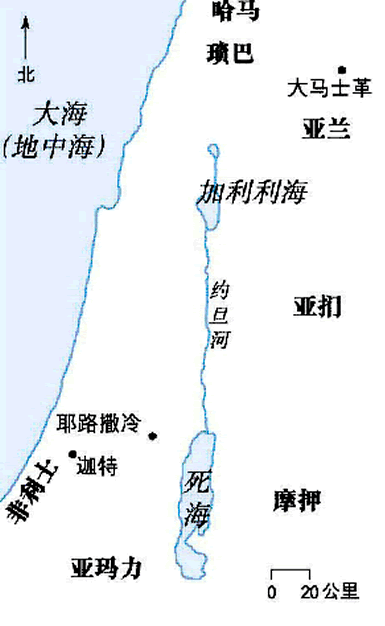
\includegraphics[width=0.4\textwidth]{BLiShiFigs/dawei}
	% \caption{大衛制服的仇敵}
	 \label{fig:1} 
	 \end{center}
	 \end{wrapfigure}
此後，大衛攻打非利士人，把他們制伏，從他們手下奪取了迦特和屬迦特的村莊。
	 
\subsubsection{敗摩押人 18:2}
又攻打摩押，摩押人就歸服大衛，給他進貢。

\subsubsection{敗瑣巴王 18:3-4}
瑣巴\footnote{撒上14:47 掃羅執掌以色列的國權，常常攻擊他四圍的一切仇敵，就是摩押人，亞捫人，以東人和瑣巴諸王，並非利士人。}\footnote{撒下8:3，代上18:3，詩60 瑣巴王哈大底謝往伯拉河去要奪回他的國權，大衛就攻打他直到哈馬，又打敗了來幫助他的大馬色的亞蘭人。}\footnote{撒下10:6，代上19:6 亞捫人知道大衛憎惡他們，就招募伯利合的亞蘭人，和瑣巴的亞蘭人來抵擋大衛，結果仍被大衛擊敗。}\footnote{撒下23:36 大衛的勇士以甲是瑣巴人。}\footnote{王上11:23 神又使以利亞大的兒子利遜興起，作所羅門的敵人，他先前逃避主人哈大底謝，大衛擊殺瑣巴人的時候，利遜招聚了一群人，自己作他們的頭目，往大馬色居住，在那裡作王，所羅門活的時候，哈達為患之外，利遜也作以色列的敵人。}王哈大利謝\footnote{在《撒下》8:3節作「哈大底謝」}往幼發拉底河去，要堅定自己的國權。大衛就攻打他，直到哈馬，奪了他的戰車一千，馬兵七千，步兵二萬，將拉戰車的馬砍斷蹄筋，但留下一百輛車的馬。

\subsubsection{敗亞蘭人 18:5-11}
大馬士革的亞蘭人來幫助瑣巴王哈大利謝，大衛就殺了亞蘭人二萬二千。 6 於是大衛在大馬士革的亞蘭地設立防營，亞蘭人就歸服他，給他進貢。大衛無論往哪裡去，耶和華都使他得勝。 7 他奪了哈大利謝臣僕所拿的金盾牌，帶到耶路撒冷。 8 大衛又從屬哈大利謝的提巴(比他)和均二城中奪取了許多的銅，後來所羅門用此製造銅海、銅柱和一切的銅器。

9 哈馬王陀烏聽見大衛殺敗瑣巴王哈大利謝的全軍， 10 就打發他兒子哈多蘭去見大衛王，問他的安，為他祝福，因為他殺敗了哈大利謝，原來陀烏與哈大利謝常常爭戰。哈多蘭帶了金銀銅的各樣器皿來。 11 大衛王將這些器皿，並從各國奪來的金銀，就是從以東、摩押、亞捫、非利士、亞瑪力人所奪來的，都分別為聖獻給耶和華。

\subsubsection{亞比篩擊以東人 18:12-13}
洗魯雅的兒子亞比篩在鹽谷擊殺了以東一萬八千人。 13 大衛在以東地設立防營，以東人就都歸服他。大衛無論往哪裡去，耶和華都使他得勝。


\subsubsection{大衛王秉公治民 18:14-17}
大衛做以色列眾人的王，又向眾民秉公行義。 15 洗魯雅的兒子約押做元帥，亞希律的兒子約沙法做史官， 16 亞希突的兒子撒督和亞比亞他的兒子亞希米勒做祭司長，沙威沙做書記， 17 耶何耶大的兒子比拿雅統轄基利提人和比利提人，大衛的眾子都在王的左右做領袖。

\subsubsection{大衛遣使詣哈嫩 19:1-5}
此後，亞捫人的王拿轄死了，他兒子接續他做王。 2 大衛說：「我要照哈嫩的父親拿轄厚待我的恩典，厚待哈嫩。」於是大衛差遣使者為他喪父安慰他。大衛的臣僕到了亞捫人的境內見哈嫩，要安慰他， 3 但亞捫人的首領對哈嫩說：「大衛差人來安慰你，你想他是尊敬你父親嗎？他的臣僕來見你不是為詳察窺探，傾覆這地嗎？」 4 哈嫩便將大衛臣僕的鬍鬚剃去一半，又割斷他們下半截的衣服，使他們露出下體，打發他們回去。 5 有人將臣僕所遇的事告訴大衛，他就差人去迎接他們，因為他們甚覺羞恥。告訴他們說：「可以住在耶利哥，等到鬍鬚長起再回來。」


\subsubsection{亞捫人備戰 19:6-9}
亞捫人知道大衛憎惡他們，哈嫩和亞捫人就打發人拿一千他連得銀子，從美索不達米亞、亞蘭瑪迦、瑣巴雇戰車和馬兵。 7 於是雇了三萬二千輛戰車和瑪迦王並他的軍兵，他們來安營在米底巴前。亞捫人也從他們的城裡出來，聚集交戰。 8 大衛聽見了，就差派約押統帶勇猛的全軍出去。 9 亞捫人出來，在城門前擺陣，所來的諸王另在郊野擺陣。


\subsubsection{亞蘭人與亞捫人敗遁 19:10-19}
約押看見敵人在他前後擺陣，就從以色列軍中挑選精兵，使他們對著亞蘭人擺陣， 11 其餘的兵交於他兄弟亞比篩，對著亞捫人擺陣。 12 約押對亞比篩說：「亞蘭人若強過我，你就來幫助我；亞捫人若強過你，我就去幫助你。 13 我們都當剛強，為本國的民和神的城邑做大丈夫！願耶和華憑他的意旨而行。」 14 於是約押和跟隨他的人前進攻打亞蘭人，亞蘭人在約押面前逃跑。 15 亞捫人見亞蘭人逃跑，他們也在約押的兄弟亞比篩面前逃跑進城。約押就回耶路撒冷去了。

16 亞蘭人見自己被以色列人打敗，就打發使者將大河那邊的亞蘭人調來，哈大利謝的將軍朔法率領他們。 17 有人告訴大衛，他就聚集以色列眾人，過約旦河，來到亞蘭人那裡，迎著他們擺陣。大衛既擺陣攻擊亞蘭人，亞蘭人就與他打仗。 18 亞蘭人在以色列人面前逃跑，大衛殺了亞蘭七千輛戰車的人、四萬步兵，又殺了亞蘭的將軍朔法。 19 屬哈大利謝的諸王見自己被以色列人打敗，就與大衛和好，歸服他。於是亞蘭人不敢再幫助亞捫人了。

\subsubsection{約押攻取拉巴 20:1-3}
過了一年，到列王出戰的時候，約押率領軍兵毀壞亞捫人的地，圍攻拉巴。大衛仍住在耶路撒冷。約押攻打拉巴，將城傾覆。 2 大衛奪了亞捫人之王(瑪勒堪」。瑪勒堪即米勒公，亞捫族之神名。)所戴的金冠冕，其上的金子重一他連得，又嵌著寶石，人將這冠冕戴在大衛頭上。大衛從城裡奪了許多財物， 3 將城裡的人拉出來，放在鋸下，或鐵耙下，或鐵斧下(強他們用鋸，或用打糧食的鐵器，或用鐵斧做工)。大衛待亞捫各城的居民都是如此。其後，大衛和眾軍都回耶路撒冷去了。

\subsubsection{三敗非利士人,殺三個迦特偉人的兒子 20:4-8}
\begin{table}[H]
\centering
\begin{tabular}{p{4.15cm}|p{4.15cm}|p{8.75cm}}\hline\hline
西比該殺基色的細派&伊勒哈難殺迦特人拉哈米 &約拿單殺迦特偉人\\\hline\hline
後來，以色列人在基色與非利士人打仗，戶沙人西比該殺了偉人的一個兒子細派，非利士人就被制伏了。
&又與非利士人打仗，睚珥的兒子伊勒哈難殺了迦特人歌利亞的兄弟拉哈米，這人的槍桿粗如織布的機軸。
&又在迦特打仗，那裡有一個身量高大的人，手腳都是六指，共有二十四個指頭，他也是偉人的兒子。這人向以色列人罵陣，大衛的哥哥示米亞的兒子約拿單就殺了他。這三個人是迦特偉人的兒子，都死在大衛和他僕人的手下。\\\hline
\end{tabular}
\end{table}


\subsubsection{大衛核數以色列民 21:1-8}
\begin{table}[H]
\centering
\begin{tabular}{p{1.25cm}|p{12.25cm}|p{3.cm}}\hline\hline
撒旦&大衛/約押&大衛禱告神\\\hline
\multirow{3}{1.4cm}{撒旦起來攻擊以色列人，激動大衛數點他們。}&大衛就吩咐約押和民中的首領說：「你們去數點以色列人，從別是巴直到但，回來告訴我，我好知道他們的數目。」&\multirow{3}{3.2cm}{神不喜悅這數點百姓的事，便降災給以色列人。大衛禱告神說：「我行這事大有罪了！現在求你除掉僕人的罪孽，因我所行的甚是愚昧。」} \\\cline{2-2}
&約押說：「願耶和華使他的百姓比現在加增百倍。我主我王啊，他們不都是你的僕人嗎？我主為何吩咐行這事？為何使以色列人陷在罪裡呢？」&\\\cline{2-2}
&但王的命令勝過約押。約押就出去，走遍以色列地，回到耶路撒冷，將百姓的總數奏告大衛。以色列人拿刀的有一百一十萬，猶大人拿刀的有四十七萬。唯有利未人和便雅憫人沒有數在其中，因為約押厭惡王的這命令。&\\\hline
\end{tabular}
\end{table}

 



\begin{table}[!hbp]
\centering
\begin{tabular}{|p{2cm}|p{1.5cm}|p{5cm}||}\hline\hline
名字   &父親名字  &職稱   \\\hline\hline
約押& 洗魯雅 &元帥 \\\hline 
約沙法  &亞希律&史官  \\\hline
撒督&亞希突&祭司長  \\\hline
亞希米勒&亞比亞他&祭司長   \\\hline
沙威沙&  &  書記  \\\hline
比拿雅&耶何耶大  & 統轄基利提人和比利提人 \\\hline
眾子&大衛  & 王的左右作領袖 \\\hline
\end{tabular}
\caption{大衛臣僕}
\end{table}


\subsubsection{耶和華怒降疫癘 21:9-17}
\begin{table}[H]
\centering
\begin{tabular}{p{5cm}|p{6.cm}|p{6.25cm}}\hline\hline
耶和華 &先見迦得  &大衛   \\\hline\hline
耶和華吩咐大衛的先見迦得說：「你去告訴大衛說：『耶和華如此說：我有三樣災，隨你選擇一樣，我好降於你。』」&於是迦得來見大衛，對他說：「耶和華如此說：『你可以隨意選擇：或三年的饑荒；或敗在你敵人面前，被敵人的刀追殺三個月；或在你國中有耶和華的刀，就是三日的瘟疫，耶和華的使者在以色列的四境施行毀滅。』現在你要想一想，我好回覆那差我來的。」&大衛對迦得說：「我甚為難。我願落在耶和華的手裡，因為他有豐盛的憐憫，我不願落在人的手裡。」\\\hline 
於是，耶和華降瘟疫於以色列人，以色列人就死了七萬。神差遣使者去滅耶路撒冷，剛要滅的時候，耶和華看見後悔，就不降這災了，吩咐滅城的天使說：「夠了，住手吧！」那時，耶和華的使者站在耶布斯人阿珥楠的禾場那裡。&  &大衛舉目，看見耶和華的使者站在天地間，手裡有拔出來的刀，伸在耶路撒冷以上。大衛和長老都身穿麻衣，面伏於地。大衛禱告神說：「吩咐數點百姓的不是我嗎？我犯了罪行了惡，但這群羊做了什麼呢？願耶和華我神的手攻擊我和我的父家，不要攻擊你的民，降瘟疫於他們。」\\\hline
\end{tabular}
\end{table}

\subsubsection{大衛築壇獻祭 21:18-31}
耶和華的使者吩咐迦得去告訴大衛，叫他上去，在耶布斯人阿珥楠的禾場上為耶和華築一座壇。 19 大衛就照著迦得奉耶和華名所說的話上去了。 20 那時阿珥楠正打麥子，回頭看見天使，就和他四個兒子都藏起來了。 21 大衛到了阿珥楠那裡，阿珥楠看見大衛，就從禾場上出去，臉伏於地，向他下拜。 22 大衛對阿珥楠說：「你將這禾場與相連之地賣給我，我必給你足價，我好在其上為耶和華築一座壇，使民間的瘟疫止住。」 23 阿珥楠對大衛說：「你可以用這禾場，願我主我王照你所喜悅的去行。我也將牛給你做燔祭，把打糧的器具當柴燒，拿麥子做素祭，這些我都送給你。」 24 大衛王對阿珥楠說：「不然，我必要用足價向你買。我不用你的物獻給耶和華，也不用白得之物獻為燔祭。」 25 於是大衛為那塊地平了六百舍客勒金子給阿珥楠。 26 大衛在那裡為耶和華築了一座壇，獻燔祭和平安祭，求告耶和華。耶和華就應允他，使火從天降在燔祭壇上。 27 耶和華吩咐使者，他就收刀入鞘。

28 那時，大衛見耶和華在耶布斯人阿珥楠的禾場上應允了他，就在那裡獻祭。 29 摩西在曠野所造之耶和華的帳幕和燔祭壇都在基遍的高處， 30 只是大衛不敢前去求問神，因為懼怕耶和華使者的刀。 [31]  大衛說：「這就是耶和華神的殿，為以色列人獻燔祭的壇。」


\subsubsection{大衛準備建聖殿 21-29}

\subsubsubsection{大衛囑以色列地的外邦人派石匠 22:1-4}  
\begin{wraptable}{r}{10cm}
\vspace{-5mm}
\centering
\begin{tabular}{p{1.25cm}|p{8cm}}\hline\hline
石匠 &聚集住以色列地的外邦人，從其中派石匠鑿石頭  \\\hline\hline
鐵&鐵做門上的釘子和鉤子\\\hline 
銅&從屬哈大利謝的提巴和均二城中奪取了許多的銅。後來所羅門用此製造銅海、銅柱，和一切的銅器。 \\\hline
香柏木&西頓人和推羅人給大衛運了許多香柏木來\\\hline\hline
\end{tabular}
\end{wraptable}	 
大衛吩咐聚集住以色列地的外邦人，從其中派石匠鑿石頭，要建造神的殿。 2 大衛預備許多鐵，做門上的釘子和鉤子；又預備許多銅，多得無法可稱； 3 又預備無數的香柏木，因為西頓人和推羅人給大衛運了許多香柏木來。 4 大衛說：「我兒子所羅門還年幼嬌嫩，要為耶和華建造的殿宇必須高大輝煌，使名譽榮耀傳遍萬國，所以我要為殿預備材料。」於是大衛在未死之先預備的材料甚多。




\subsubsubsection{大衛囑所羅門為主建殿 22:5-15}  
\begin{table}[H]
\vspace{-5mm}
\hspace{-10mm}
\centering
\begin{tabular}{p{4.2cm}|p{4.cm}|p{4.25cm}|p{4.05cm}}\hline\hline
不许大衛建殿&對所羅門的應許&贈言所羅門&大衛為建殿的預備\\\hline
大衛召了他兒子所羅門來，囑咐他給耶和華以色列的神建造殿宇，對所羅門說：「我兒啊，我心裡本想為耶和華我神的名建造殿宇，只是耶和華的話臨到我說：『你流了多人的血，打了多次大仗，你不可為我的名建造殿宇，因為你在我眼前使多人的血流在地上。 
&你要生一個兒子，他必做太平的人。我必使他安靜，不被四圍的仇敵擾亂。他的名要叫所羅門(太平)，他在位的日子，我必使以色列人平安康泰。他必為我的名建造殿宇。他要做我的子，我要做他的父。他做以色列王，我必堅定他的國位直到永遠。』
&我兒啊，現今願耶和華與你同在，使你亨通，照他指著你說的話，建造耶和華你神的殿。但願耶和華賜你聰明、智慧，好治理以色列國，遵行耶和華你神的律法。你若謹守遵行耶和華藉摩西吩咐以色列的律例、典章，就得亨通。你當剛強壯膽，不要懼怕，也不要驚惶。
&我在困難之中為耶和華的殿預備了金子十萬他連得，銀子一百萬他連得，銅和鐵多得無法可稱。我也預備了木頭、石頭，你還可以增添。你有許多匠人，就是石匠、木匠和一切能做各樣工的巧匠，並有無數的金、銀、銅、鐵。你當起來辦事，願耶和華與你同在。」\\\hline
\end{tabular}
\end{table}	 

\subsubsubsection{大衛囑以色列的眾首領 22:16-19} 
大衛又吩咐以色列的眾首領幫助他兒子所羅門，說： 17 「耶和華你們的神不是與你們同在嗎？不是叫你們四圍都平安嗎？因他已將這地的居民交在我手中，這地就在耶和華與他百姓面前制伏了。 18 現在你們應當立定心意，尋求耶和華你們的神，也當起來建造耶和華神的聖所，好將耶和華的約櫃和供奉神的聖器皿都搬進為耶和華名建造的殿裡。」


\subsubsection{利未人的職責 23}

\subsubsubsection{三十歲以外的利未人 23:1-6}
%\begin{minipage}{.5\textwidth} %
\begin{wraptable}{r}{6cm}
\vspace{-15mm}
\centering
\begin{tabular}{p{3cm}|p{1.cm}}\hline\hline
利未人& 數目 \\\hline
三十歲以外(總數）& 38,000 \\\hline
管理耶和華殿的&24,000 \\\hline
官長和士師&6,000\\\hline
作守門的&4,000\\\hline
用樂器頌讚耶和華&4,000\\\hline
\end{tabular}
\end{wraptable}	 
大衛年紀老邁，日子滿足，就立他兒子所羅門做以色列的王。大衛招聚以色列的眾首領和祭司、利未人。 3 利未人從三十歲以外的都被數點，他們男丁的數目共有三萬八千。 4 其中有二萬四千人管理耶和華殿的事，有六千人做官長和士師， 5 有四千人做守門的，又有四千人用大衛所做的樂器頌讚耶和華。 6 大衛將利未人革順、哥轄、米拉利的子孫分了班次。


\subsubsubsection{革順子孫的族長 23:7-11}
\begin{figure}[H]
\begin{minipage}{.4\textwidth} %
 \begin{forest}
  for tree={
    child anchor=west,
    parent anchor=east,
    grow=east,
    draw,
    anchor=west,
    edge path={
      \noexpand\path[\forestoption{edge}]
        (.child anchor) -| +(-5pt,0) -- +(-5pt,0) |-
        (!u.parent anchor)\forestoption{edge label};
    },
  }
  [革順[拉但[耶歇][細坦][約珥]]
       [示每[雅哈(長子)][細拿(次子)][耶烏施][比利亞]]  
  ]
\end{forest}
\end{minipage}
\begin{minipage}{.4\textwidth} %
革順的子孫有拉但和示每。 8 拉但的長子是耶歇，還有細坦和約珥，共三人。 9 示每的兒子是示羅密、哈薛、哈蘭三人。這是拉但族的族長。 10 示每的兒子是雅哈、細拿、耶烏施、比利亞，共四人。 11 雅哈是長子，細撒是次子，但耶烏施和比利亞的子孫不多，所以算為一族。
\end{minipage}
\end{figure}

\subsubsubsection{革轄子孫的族長 23:12-20}
\begin{figure}[H]
\begin{minipage}{.5\textwidth} %
\begin{forest}
  for tree={
    child anchor=west,
    parent anchor=east,
    grow=east,
    draw,
    anchor=west,
    edge path={
      \noexpand\path[\forestoption{edge}]
        (.child anchor) -| +(-5pt,0) -- +(-5pt,0) |-
        (!u.parent anchor)\forestoption{edge label};
    },
  }
  [哥轄[暗蘭[亞倫][摩西[革舜[細布業]][以利以謝[利哈比雅[伊示雅]]]][?[書巴業[耶希底亞]]]]
       [以斯哈[示羅密[雅哈]]] 
       [希伯倫[耶利雅][亞瑪利亞][雅哈悉][耶加面]]
       [烏薛[米迦[沙密]][耶西雅[撒迦利雅]]] 
  ]
\end{forest}
\end{minipage}
\begin{minipage}{.5\textwidth} %
\vspace{-15mm}
哥轄的兒子是暗蘭、以斯哈、希伯倫、烏薛，共四人。 13 暗蘭的兒子是亞倫、摩西。亞倫和他的子孫分出來，好分別至聖的物，在耶和華面前燒香，侍奉他，奉他的名祝福，直到永遠。 14 至於神人摩西，他的子孫名字記在利未支派的冊上。 15 摩西的兒子是革舜和以利以謝。 16 革舜的長子是細布業。 17 以利以謝的兒子是利哈比雅。以利以謝沒有別的兒子，但利哈比雅的子孫甚多。 18 以斯哈的長子是示羅密。 19 希伯倫的長子是耶利雅，次子是亞瑪利亞，三子是雅哈悉，四子是耶加面。 20 烏薛的長子是米迦，次子是耶西雅。
\end{minipage}
\end{figure}

\subsubsubsection{米拉利子孫的族長 23:21-23}
\begin{figure}[H]
\begin{minipage}{.3\textwidth} %
\begin{forest}
  for tree={
    child anchor=west,
    parent anchor=east,
    grow=east,
    draw,
    anchor=west,
    edge path={
      \noexpand\path[\forestoption{edge}]
        (.child anchor) -| +(-5pt,0) -- +(-5pt,0) |-
        (!u.parent anchor)\forestoption{edge label};
    },
  }
  [米拉利[抹利[以利亞撒][基士[耶拉篾]]]
         [母示[末力][以得][耶利摩]]
         [雅西雅[比挪][朔含][撒刻][伊比利]]  
  ]
\end{forest}
\end{minipage}
\begin{minipage}{.4\textwidth} %
米拉利的兒子是抹利、母示。抹利的兒子是以利亞撒、基士。 22 以利亞撒死了，沒有兒子，只有女兒，他們本族基士的兒子娶了她們為妻。 23 母示的兒子是末力、以得、耶利摩，共三人。
\end{minipage}
\end{figure}

\subsubsubsection{二十歲以外的利未人職責 23:24-32}
\begin{table}[H]
\centering
\vspace{-5mm}
\begin{tabular}{p{6.5cm}|p{10.5cm}}\hline\hline
大衛的臨終吩咐&利未人職責\\\hline 
\multirow{8}{6.6cm}{以上利未子孫做族長的，照著男丁的數目，從二十歲以外，都辦耶和華殿的事務。大衛說：「耶和華以色列的神已經使他的百姓平安，他永遠住在耶路撒冷。利未人不必再抬帳幕和其中所用的一切器皿了。」照著大衛臨終所吩咐的，利未人從二十歲以外的都被數點。他們的職任是：}&服侍亞倫的子孫，\\\cline{2-2}
&在耶和華的殿和院子並屋中辦事，潔淨一切聖物，就是辦神殿的事務；\\\cline{2-2}
&並管理陳設餅，素祭的細麵，或無酵薄餅，或用盤烤或用油調和的物，\\\cline{2-2} 
&又管理各樣的升斗尺度；\\\cline{2-2} 
&每日早晚，站立稱謝讚美耶和華；\\\cline{2-2}
&又在安息日、月朔並節期，按數照例，將燔祭常常獻給耶和華；\\\cline{2-2}
&又看守會幕和聖所，\\\cline{2-2}
&並守耶和華吩咐他們弟兄亞倫子孫的，辦耶和華殿的事。\\\hline 
\end{tabular}
\end{table}	 


\subsubsection{祭司的24班次 24}
\subsubsubsection{祭司的後裔 24:1-6}
亞倫子孫的班次記在下面。亞倫的兒子是拿答、亞比戶、以利亞撒、以他瑪。 2 拿答、亞比戶死在他們父親之先，沒有留下兒子，故此以利亞撒、以他瑪供祭司的職分。 3 以利亞撒的子孫撒督和以他瑪的子孫亞希米勒，同著大衛將他們的族弟兄分成班次。 4 以利亞撒子孫中為首的比以他瑪子孫中為首的更多，分班如下：以利亞撒的子孫中有十六個族長，以他瑪的子孫中有八個族長； 5 都掣籤分立，彼此一樣，在聖所和神面前做首領的有以利亞撒的子孫，也有以他瑪的子孫。 6 做書記的利未人拿坦業的兒子示瑪雅，在王和首領與祭司撒督，亞比亞他的兒子亞希米勒，並祭司、利未人的族長面前記錄他們的名字，在以利亞撒的子孫中取一族，在以他瑪的子孫中取一族。

\subsubsubsection{祭司的班次 24:7-19}
\begin{table}[!hbp]
\centering
\begin{tabular}{p{2cm}|p{1.5cm}|p{2cm}|p{1.3cm}|p{2cm}|p{1.5cm}|p{1.9cm}|p{1.3cm}}\hline\hline
第一掣  &耶何雅立  & 第二掣 &耶大雅  & 第三掣 &哈琳&第四掣& 梭琳\\\hline
第五掣  &瑪基雅  & 第六掣 &米雅民  & 第七掣 &哈歌斯&第八掣&亞比雅\\\hline
第九掣  &耶書亞  & 第十掣 &示迦尼  & 第十一掣 &以利亞實&第十二掣&雅金\\\hline
第十三掣  &胡巴  & 第十四掣 &比押  & 第十五掣 &璧迦&第十六掣&音麥\\\hline
第十七掣  &希悉  & 第十八掣 &哈闢悉  & 第十九掣 &毗他希雅&第二十掣&以西結\\\hline
第二十一掣  &雅斤  & 第二十二掣 &迦末  & 第二十三掣 &第來雅&第二十四掣&瑪西亞\\\hline
\end{tabular}
\end{table}	 
掣籤的時候，第一掣出來的是耶何雅立，第二是耶大雅， 8 第三是哈琳，第四是梭琳， 9 第五是瑪基雅，第六是米雅民， 10 第七是哈歌斯，第八是亞比雅， 11 第九是耶書亞，第十是示迦尼， 12 第十一是以利亞實，第十二是雅金， 13 第十三是胡巴，第十四是耶是比押， 14 第十五是璧迦，第十六是音麥， 15 第十七是希悉，第十八是哈闢悉， 16 第十九是毗他希雅，第二十是以西結， 17 第二十一是雅斤，第二十二是迦末， 18 第二十三是第來雅，第二十四是瑪西亞。 19 這就是他們的班次，要照耶和華以色列的神藉他們祖宗亞倫所吩咐的條例，進入耶和華的殿辦理事務。

\subsubsubsection{其餘利未之裔亦掣籤得職 24:20-31}
利未其餘的子孫如下：暗蘭的子孫裡有書巴業，書巴業的子孫裡有耶希底亞， 21 利哈比雅的子孫裡有長子伊示雅； 22 以斯哈的子孫裡有示羅摩，示羅摩的子孫裡有雅哈； 23 希伯倫的子孫裡有長子耶利雅，次子亞瑪利亞，三子雅哈悉，四子耶加面； 24 烏薛的子孫裡有米迦，米迦的子孫裡有沙密， 25 米迦的兄弟是伊示雅，伊示雅的子孫裡有撒迦利雅。 26 米拉利的兒子是抹利、母示、雅西雅。雅西雅的兒子有比挪， 27 米拉利的子孫裡有雅西雅的兒子比挪、朔含、撒刻、伊比利； 28 抹利的兒子是以利亞撒，以利亞撒沒有兒子， 29 基士的子孫裡有耶拉篾； 30 母示的兒子是末力、以得、耶利摩。按著宗族，這都是利未的子孫。 31 他們在大衛王和撒督並亞希米勒，與祭司、利未人的族長面前掣籤，正如他們弟兄亞倫的子孫一般，各族的長者與兄弟沒有分別。

\subsubsection{神殿中的聖樂的24班次 25}
\subsubsubsection{神殿中的聖樂者 25:1-8}
大衛和眾首領分派亞薩、希幔並耶杜頓的子孫彈琴、鼓瑟、敲鈸、唱歌(原文作「說預言」)。他們供職的人數記在下面： 2 亞薩的兒子撒刻、約瑟、尼探雅、亞薩利拉，都歸亞薩指教，遵王的旨意唱歌。 3 耶杜頓的兒子基大利、西利、耶篩亞、哈沙比雅、瑪他提雅、示每，共六人，都歸他們父親耶杜頓指教，彈琴唱歌，稱謝、頌讚耶和華。 4 希幔的兒子布基雅、瑪探雅、烏薛、細布業、耶利摩、哈拿尼雅、哈拿尼、以利亞他、基大利提、羅幔提以謝、約施比加沙、瑪羅提、何提、瑪哈秀， 5 這都是希幔的兒子，吹角頌讚。希幔奉神之命做王的先見。神賜給希幔十四個兒子、三個女兒， 6 都歸他們父親指教，在耶和華的殿唱歌、敲鈸、彈琴、鼓瑟，辦神殿的事務。亞薩、耶杜頓、希幔都是王所命定的。 7 他們和他們的弟兄學習頌讚耶和華，善於歌唱的共有二百八十八人。 8 這些人，無論大小，為師的為徒的，都一同掣籤分了班次。

\subsubsubsection{神殿中的聖樂的班次 25:9-31}
\begin{figure}[H]
\begin{minipage}{.5\textwidth} %
\begin{forest}
  for tree={
    child anchor=west,
    parent anchor=east,
    grow=east,
    draw,
    anchor=west,
    edge path={
      \noexpand\path[\forestoption{edge}]
        (.child anchor) -| +(-5pt,0) -- +(-5pt,0) |-
        (!u.parent anchor)\forestoption{edge label};
    },
  }
  [聖詩班[亞薩(唱歌)[撒刻3][約瑟1][尼探雅5][亞薩利拉都(7?)]]
    		[耶杜頓(彈琴，唱歌，稱謝頌讚耶和華)[基大利2][西利(4?)][耶篩亞8][哈沙比雅12]
    														[瑪他提雅14][示每10]]
  		 	[希幔(吹角)[布基雅6][瑪探雅9][烏薛(11?)][細布業(13?)][耶利摩15][哈拿尼雅16]
  		 	[哈拿尼18][以利亞他20][基大利提22][羅幔提以謝24][約施比加沙17][瑪羅提19]
  		 				  [何提21][瑪哈秀23]]
  ]
\end{forest}
\end{minipage}
\hspace{-20mm}
\begin{minipage}{.55\textwidth} %
\vspace{-60mm}
掣籤的時候，第一掣出來的是亞薩的兒子約瑟；第二是基大利，他和他弟兄並兒子，共十二人； 10 第三是撒刻，他和他兒子並弟兄，共十二人； 11 第四是伊洗利，他和他兒子並弟兄，共十二人； 12 第五是尼探雅，他和他兒子並弟兄，共十二人； 13 第六是布基雅，他和他兒子並弟兄，共十二人； 14 第七是耶薩利拉，他和他兒子並弟兄，共十二人； 15 第八是耶篩亞，他和他兒子並弟兄，共十二人； 16 第九是瑪探雅，他和他兒子並弟兄，共十二人； 17 第十是示每，他和他兒子並弟兄，共十二人； 18 第十一是亞薩烈，他和他兒子並弟兄，共十二人； 19 第十二是哈沙比雅，他和他兒子並弟兄，共十二人； 20 第十三是書巴業，他和他兒子並弟兄，共十二人； 21 第十四是瑪他提雅，他和他兒子並弟兄，共十二人； 22 第十五是耶利摩，他和他兒子並弟兄，共十二人； 23 第十六是哈拿尼雅，他和他兒子並弟兄，共十二人； 24 第十七是約施比加沙，他和他兒子並弟兄，共十二人； 25 第十八是哈拿尼，他和他兒子並弟兄，共十二人； 26 第十九是瑪羅提，他和他兒子並弟兄，共十二人； 27 第二十是以利亞他，他和他兒子並弟兄，共十二人； 28 第二十一是何提，他和他兒子並弟兄，共十二人； 29 第二十二是基大利提，他和他兒子並弟兄，共十二人； 30 第二十三是瑪哈秀，他和他兒子並弟兄，共十二人； 31 第二十四是羅幔提以謝，他和他兒子並弟兄，共十二人。
\end{minipage}
\end{figure}




\subsubsection{神殿中的守門的班次 26:1-19}
\begin{figure}[H]
\begin{minipage}{.7\textwidth} %
\begin{forest}
  for tree={
    child anchor=west,
    parent anchor=east,
    grow=east,
    draw,
    anchor=west,
    edge path={
      \noexpand\path[\forestoption{edge}]
        (.child anchor) -| +(-5pt,0) -- +(-5pt,0) |-
        (!u.parent anchor)\forestoption{edge label};
    },
  }
  [守門班次[可拉族[亞薩[可利[米施利米雅（18人）[撒迦利亞][耶疊][西巴第雅]
   			                            [耶提聶][以攔][約哈難][以利約乃]]
    		                   [俄別以東(62人）[示瑪雅[俄得尼][利法益][俄備得]
    		                                          [以利薩巴][以利戶][西瑪迦]]
    				                             [約薩拔][約亞][沙甲][拿坦業]
    				                             [亞米利][以薩迦][毗烏利太]]]]]
  		 	[米拉利[何薩（13人）[申利][希勒家][底巴利雅][撒迦利亞]]]
  ]
\end{forest}
\end{minipage}
\hspace{10mm}
\begin{minipage}{.25\textwidth} %
\vspace{0mm}
守門的班次記在下面：可拉族亞薩的子孫中，有可利的兒子米施利米雅。 2 米施利米雅的長子是撒迦利亞，次子是耶疊，三子是西巴第雅，四子是耶提聶， 3 五子是以攔，六子是約哈難，七子是以利約乃。 4 俄別以東的長子是示瑪雅，次子是約薩拔，三子是約亞，四子是沙甲，五子是拿坦業， 5 六子是亞米利，七子是以薩迦，八子是毗烏利太，因為神賜福於俄別以東。 6 他的兒子示瑪雅有幾個兒子，都是大能的壯士，掌管父親的家。 7 示瑪雅的兒子是俄得尼、利法益、俄備得、以利薩巴，以利薩巴的弟兄是壯士，還有以利戶和西瑪迦。 8 這都是俄別以東的子孫，他們和他們的兒子並弟兄都是善於辦事的壯士，俄別以東的子孫共六十二人。 9 米施利米雅的兒子和弟兄都是壯士，共十八人。 10 米拉利子孫何薩有幾個兒子，長子是申利（他原不是長子，是他父親立他做長子）， 11 次子是希勒家，三子是底巴利雅，四子是撒迦利亞。何薩的兒子並弟兄共十三人。
\end{minipage}
\end{figure}

\begin{wrapfigure}{r}{.7\textwidth}
\begin{tikzpicture}
  [node distance=.4cm,
  start chain=going below,]
     \node[punktchain, join] (intro) {撒迦利亞(北)};   
     \node (asym) [punktchain ]  {\textcolor{red}{聖殿}};
      \begin{scope}[start branch=venstre,
        %We need to redefine the join-style to have the -> turn out right
       % every join/.style={->, thick, shorten <=1pt}, ]
       every join/.style={  thick, shorten <=1pt}, ]
        %\node[punktchain, on chain=going left, join=by {<-}](risiko) {阿土};
   \node[punktchain, on chain=going left](risiko) {書聘與何薩(西)};
      \end{scope}
      \begin{scope}[start branch=hoejre,]
  \node (finans) [punktchain, on chain=going right] {示利米雅(東)};
    \end{scope}
  %\node[punktchain, join] (disk) {俄別以東(南門)};
   % \node[punktchain, join] (intro) {俄別以東(南門)};
        \node (asym) [punktchain ]  {俄別以東(南)};
  \end{tikzpicture}
\end{wrapfigure}
這些人都是守門的班長，與他們的弟兄一同在耶和華殿裡，按班供職。 13 他們無論大小，都按著宗族掣籤，分守各門。 14 掣籤守東門的是示利米雅。他的兒子撒迦利亞是精明的謀士，掣籤守北門。 15 俄別以東守南門，他的兒子守庫房。 16 書聘與何薩守西門，在靠近沙利基門通著往上去的街道上，班與班相對。 17 每日東門有六個利未人，北門有四個，南門有四個，庫房有兩個，又有兩個輪班替換， 18 在西面街道上有四個，在遊廊上有兩個。 19 以上是可拉子孫和米拉利子孫守門的班次。

\subsubsection{掌管神殿的府庫和聖物的府庫班次 26:20-32}
\begin{figure}[H]
\begin{minipage}{.7\textwidth} %
\begin{tikzpicture}[every node/.style={circle,draw},level 1/.style={sibling distance=35mm},level 2/.style={sibling distance=30mm},level 3/.style={sibling distance=20mm}
]
\node {府庫}
child { node {革順} 
%child { node {E} }
child { node {拉但}  child { node {耶希伊利}child { node {西坦} }child { node {約珥} } } }}
child { node {亞希雅}}
child { node {哥轄} child {node {暗蘭} child {node {摩西}child {node {革舜}child {node {細布業}}child { node {以利以謝}child { node {利哈比雅}child { node {耶篩亞}child { node {約蘭}child { node {細基利}child { node {示羅密} } } } } } }}} }
                    child {node {希伯倫}child {node {哈沙比雅} }child {node {耶利雅} }}
                    child {node {烏泄}} 
                    child {node {以斯哈}child {node {基拿尼雅} } }}
;
\end{tikzpicture}
\end{minipage}
\hspace{-60mm}
\begin{minipage}{.6\textwidth} %
\vspace{60mm}
\begin{itemize}
\item 掌府庫之利未人\\
利未子孫中有亞希雅掌管神殿的府庫和聖物的府庫。 21 革順族拉但子孫裡做族長的是革順族拉但的子孫耶希伊利， 22 耶希伊利的兒子西坦和他兄弟約珥掌管耶和華殿裡的府庫。 23 暗蘭族、以斯哈族、希伯倫族、烏薛族也有職分。 24 摩西的孫子、革舜的兒子細布業掌管府庫。 25 還有他的弟兄以利以謝，以利以謝的兒子是利哈比雅，利哈比雅的兒子是耶篩亞，耶篩亞的兒子是約蘭，約蘭的兒子是細基利，細基利的兒子是示羅密， 26 這示羅密和他的弟兄掌管府庫的聖物，就是大衛王和眾族長、千夫長、百夫長並軍長所分別為聖的物。 27 他們將爭戰時所奪的財物分別為聖，以備修造耶和華的殿。 28 先見撒母耳、基士的兒子掃羅、尼珥的兒子押尼珥、洗魯雅的兒子約押所分別為聖的物，都歸示羅密和他的弟兄掌管。
\item 做官長士師之利未人\\
以斯哈族有基拿尼雅和他眾子做官長和士師，管理以色列的外事。 30 希伯倫族有哈沙比雅和他弟兄一千七百人，都是壯士，在約旦河西以色列地辦理耶和華與王的事。 31 希伯倫族中有耶利雅做族長（大衛做王第四十年，在基列的雅謝，從這族中尋得大能的勇士）， 32 耶利雅的弟兄有二千七百人，都是壯士，且做族長。大衛王派他們在魯本支派、迦得支派、瑪拿西半支派中辦理神和王的事。
\end{itemize}
\end{minipage}
\end{figure}



\subsubsection{軍事長官的班次 27:1-15}
\begin{table}[H]
\centering
\begin{tabular}{p{1.5cm}|p{4.5cm}|p{2.3cm}|p{1.1cm}|p{3.2cm}}\hline\hline
月份    &班長                  & 父親名字      & 人數  & 支派  \\\hline
第一月  &雅朔班                & 撒巴第業     &24,000 & 法勒斯的子孫\\\hline
第二月  &朵代,副官密基羅       &             &24,000 &亞哈希人 \\\hline
第三月  &比拿雅(30勇士中的首領)& 祭司耶何耶大 &24,000 & \\\hline
第四月  &亞撒黑(兒子西巴第雅接續)  & 約押的兄弟   & 24,000 &猶大\\\hline
第五月  &珊合 &   &24,000&伊斯拉人\\\hline
第六月  &以拉  &益吉  &24,000 &提哥亞人  \\\hline
 第七月 &希利斯&  &24,000 &以法蓮族比倫人\\\hline
 第八月& 西比該 &  &24,000 &謝拉族戶沙人\\\hline
 第九月 &亞比以謝 &  &24,000&便雅憫族亞拿突人\\\hline
 第十月&瑪哈萊 &  &24,000& 謝拉族尼陀法人\\\hline
 第十一月&比拿雅 &  &24,000&  以法蓮族比拉頓人\\\hline
 第十二月  &黑玳 &  &24,000&  俄陀聶族尼陀法人 \\\hline
\end{tabular}
\end{table}	 
以色列人的族長、千夫長、百夫長和官長都分定班次，每班是二萬四千人，週年按月輪流，替換出入服侍王。 2 正月第一班的班長是撒巴第業的兒子雅朔班，他班內有二萬四千人。 3 他是法勒斯的子孫，統管正月班的一切軍長。 4 二月的班長是亞合人朵代，還有副官密基羅，他班內有二萬四千人。 5 三月第三班的班長(軍長)是祭司耶何耶大的兒子比拿雅，他班內有二萬四千人。 6 這比拿雅是那三十人中的勇士，管理那三十人，他班內又有他兒子暗米薩拔。 7 四月第四班的班長是約押的兄弟亞撒黑，接續他的是他兒子西巴第雅，他班內有二萬四千人。 8 五月第五班的班長是伊斯拉人珊合，他班內有二萬四千人。 9 六月第六班的班長是提哥亞人益吉的兒子以拉，他班內有二萬四千人。 10 七月第七班的班長是以法蓮族比倫人希利斯，他班內有二萬四千人。 11 八月第八班的班長是謝拉族戶沙人西比該，他班內有二萬四千人。 12 九月第九班的班長是便雅憫族亞拿突人亞比以謝，他班內有二萬四千人。 13 十月第十班的班長是謝拉族尼陀法人瑪哈萊，他班內有二萬四千人。 14 十一月第十一班的班長是以法蓮族比拉頓人比拿雅，他班內有二萬四千人。 15 十二月第十二班的班長是俄陀聶族尼陀法人黑玳，他班內有二萬四千人。

\subsubsection{管理以色列眾支派的 27:16-24} 
\begin{wraptable}{r}{9cm}
\centering
\begin{tabular}{p{3.5cm}|p{2.cm}|p{2.6cm}}\hline\hline
支派        &首領          & 父親名字        \\\hline
流便  &以利以謝               &細基利\\\hline
西緬  &示法提雅 &瑪迦 \\\hline
利未  &哈沙比雅 &基母利 \\\hline
亞倫子孫  &撒督& \\\hline
猶大 &  以利戶 &大衛的一個哥哥\\\hline
以薩迦  &暗利  &米迦勒  \\\hline
 西布倫  &伊施瑪雅 &俄巴第雅\\\hline
 拿弗他利 & 耶利摩 &亞斯列\\\hline
 以法蓮&何細亞 &阿撒細雅\\\hline
 瑪拿西半支派&約珥  &毗大雅\\\hline
 基列地瑪拿西半支派&易多 &  撒迦利亞\\\hline
 便雅憫 &雅西業& 押尼珥 \\\hline
 但 &亞薩列& 耶羅罕\\\hline
\end{tabular}
\end{wraptable}
管理以色列眾支派的記在下面：管魯本人的，是細基利的兒子以利以謝；管西緬人的，是瑪迦的兒子示法提雅； 17 管利未人的，是基母利的兒子哈沙比雅；管亞倫子孫的，是撒督； 18 管猶大人的，是大衛的一個哥哥以利戶；管以薩迦人的，是米迦勒的兒子暗利； 19 管西布倫人的，是俄巴第雅的兒子伊施瑪雅；管拿弗他利人的，是亞斯列的兒子耶利摩； 20 管以法蓮人的，是阿撒細雅的兒子何細亞；管瑪拿西半支派的，是毗大雅的兒子約珥； 21 管基列地瑪拿西那半支派的，是撒迦利亞的兒子易多；管便雅憫人的，是押尼珥的兒子雅西業； 22 管但人的，是耶羅罕的兒子亞薩列。以上是以色列眾支派的首領。 23 以色列人二十歲以內的，大衛沒有記其數目，因耶和華曾應許說必加增以色列人如天上的星那樣多。 24 洗魯雅的兒子約押動手數點，當時耶和華的烈怒臨到以色列人，因此沒有點完，數目也沒有寫在《大衛王記》上。

\subsubsection{大衛諸臣及其職守 27:25-34}
\begin{table}[H]
\centering
\begin{tabular}{p{3.5cm}|p{5.3cm}|p{4.3cm}}\hline\hline
長官                    & 職責  & 備註  \\\hline
押斯馬威  &掌管王府庫    &亞疊的兒子\\\hline
約拿單  &掌管田野城邑村莊保障之倉庫           &烏西雅的兒子 \\\hline
以斯利  &掌管耕田種地& 基綠的兒子 \\\hline
示每  &掌管葡萄園& 拉瑪人\\\hline
撒巴底  &掌管葡萄園酒窖&實弗米人\\\hline
巴勒哈南  &掌管高原橄欖樹和桑樹  &基第利人  \\\hline
 約阿施 &掌管油庫 &\\\hline
 施提賚& 掌管沙崙牧放牛群 &沙崙人\\\hline
 沙法 &掌管山谷牧養牛群 &亞第賚的兒子\\\hline
 阿比勒&掌管駝群&以實瑪利人\\\hline
 耶希底亞&掌管驢群& 米崙人\\\hline
 雅悉  &掌管羊群& 夏甲人 \\\hline
 約拿單&作謀士,又作書記& 大衛的叔叔,這人有智慧\\\hline
 耶歇&作王眾子的師傅&哈摩尼的兒子\\\hline
 亞希多弗&作謀士&\\\hline
 戶篩&作王的陪伴&亞基人\\\hline
耶何耶大和亞比亞他&接續戶篩作謀士&耶何耶大是比拿雅的兒子\\\hline
\end{tabular}
%\caption{管理王產業的長官}
\end{table}	 
掌管王府庫的，是亞疊的兒子押斯馬威；掌管田野城邑村莊保障之倉庫的，是烏西雅的兒子約拿單； 26 掌管耕田種地的，是基綠的兒子以斯利； 27 掌管葡萄園的，是拉瑪人示每；掌管葡萄園酒窖的，是實弗米人撒巴底； 28 掌管高原橄欖樹和桑樹的，是基第利人巴勒哈南；掌管油庫的，是約阿施； 29 掌管沙崙牧放牛群的，是沙崙人施提賚；掌管山谷牧養牛群的，是亞第賚的兒子沙法； 30 掌管駝群的，是以實瑪利人阿比勒；掌管驢群的，是米崙人耶希底亞；掌管羊群的，是夏甲人雅悉。 31 這都是給大衛王掌管產業的。

32 大衛的叔叔約拿單做謀士，這人有智慧，又做書記。哈摩尼的兒子耶歇做王眾子的師傅。 33 亞希多弗也做王的謀士。亞基人戶篩做王的陪伴。 34 亞希多弗之後，有比拿雅的兒子耶何耶大和亞比亞他接續他做謀士。約押做王的元帥。


\subsubsection{大衛關於建殿的指示 28}
\subsubsubsection{大衛集眾宣述建殿之意 28:1-8}
\begin{table}[H]
\centering
\begin{tabular}{p{2.75cm}|p{14.cm}}\hline\hline
\multirow{4}{2.86cm}{大衛招聚以色列各支派的首領和輪班服侍王的軍長，與千夫長、百夫長，掌管王和王子產業牲畜的，並太監，以及大能的勇士，都到耶路撒冷來。 2 大衛王就站起來，說：}
&我的弟兄，我的百姓啊，你們當聽我言。我心裡本想建造殿宇，安放耶和華的約櫃，作為我神的腳凳，我已經預備建造的材料， 3 只是神對我說：『你不可為我的名建造殿宇，因你是戰士，流了人的血。』\\\cline{2-2}
&然而，耶和華以色列的神在我父的全家揀選我做以色列的王，直到永遠。因他揀選猶大為首領，在猶大支派中揀選我父家，在我父的眾子裡喜悅我，立我做以色列眾人的王。 5 耶和華賜我許多兒子，在我兒子中揀選所羅門坐耶和華的國位，治理以色列人。 6 耶和華對我說：『你兒子所羅門必建造我的殿和院宇，因為我揀選他做我的子，我也必做他的父。 7 他若恆久遵行我的誡命、典章，如今日一樣，我就必堅定他的國位直到永遠。』\\\cline{2-2}
&現今，在耶和華的會中、以色列眾人眼前所說的，我們的神也聽見了，你們應當尋求耶和華你們神的一切誡命，謹守遵行，如此你們可以承受這美地，遺留給你們的子孫永遠為業。\\\hline
\end{tabular}
%\caption{大衛關於建殿的指示}
\end{table}	 


\subsubsubsection{以聖殿模式示所羅門 28:9-21}
\begin{table}[H]
\centering
\begin{tabular}{p{3.cm}|p{9.5cm}|p{4.cm}}\hline\hline
\multirow{4}{3.1cm}{我兒所羅門哪，你當認識耶和華你父的神，誠心樂意地侍奉他，因為他鑒察眾人的心，知道一切心思意念。你若尋求他，他必使你尋見；你若離棄他，他必永遠丟棄你。你當謹慎，因耶和華揀選你建造殿宇作為聖所。你當剛強去行。}
&大衛將殿的遊廊、旁屋、府庫、樓房、內殿和施恩所的樣式指示他兒子所羅門。又將被靈感動所得的樣式，就是耶和華神殿的院子、周圍的房屋、殿的府庫和聖物府庫的一切樣式，都指示他。&\multirow{4}{4.1cm}{大大衛又對他兒子所羅門說：「你當剛強壯膽去行，不要懼怕，也不要驚惶。因為耶和華神，就是我的神，與你同在，他必不撇下你，也不丟棄你，直到耶和華殿的工作都完畢了。有祭司和利未人的各班，為要辦理神殿各樣的事，又有靈巧的人在各樣的工作上樂意幫助你，並有眾首領和眾民一心聽從你的命令。}\\\cline{2-2}
&又指示他祭司和利未人的班次，與耶和華殿裡各樣的工作，&\\\cline{2-2}
&並耶和華殿裡一切器皿的樣式，以及各樣應用金器的分量和各樣應用銀器的分量，金燈臺和金燈的分量，銀燈臺和銀燈的分量（輕重各都合宜），陳設餅金桌子的分量，銀桌子的分量，精金的肉叉子、盤子和爵的分量，各金碗與各銀碗的分量，精金香壇的分量，&\\\cline{2-2}
&並用金子做基路伯(用金子作車式的基路伯)，基路伯張開翅膀，遮掩耶和華的約櫃。大衛說：「這一切工作的樣式，都是耶和華用手劃出來使我明白的。」&\\\hline
\end{tabular}
\end{table}	 


\begin{table}[H]
\centering
\begin{tabular}{p{2.75cm}|p{10.cm}|p{3.9m}}\hline\hline

%&又指示他祭司和利未人的班次，與耶和華殿裡各樣的工作，&\\\cline{2-2}
%&並耶和華殿裡一切器皿的樣式，以及各樣應用金器的分量和各樣應用銀器的分量，金燈臺和金燈的分量，銀燈臺和銀燈的分量（輕重各都合宜），陳設餅金桌子的分量，銀桌子的分量，精金的肉叉子、盤子和爵的分量，各金碗與各銀碗的分量，精金香壇的分量，&\\\cline{2-2}
%&並用金子做基路伯(用金子作車式的基路伯)，基路伯張開翅膀，遮掩耶和華的約櫃。大衛說：「這一切工作的樣式，都是耶和華用手劃出來使我明白的。」&\\\hline
\end{tabular}
\end{table}	 





\subsubsection{大衛及眾人為建殿而獻的禮物 29}
\begin{table}[H]
\centering
\begin{tabular}{|p{1cm}|p{4cm}|p{2.1cm}|p{1.3cm}|p{2.3cm}|p{2.3cm}|}\hline\hline
     &金 (他連得)       &銀 (他連得)          &銅&鐵&寶石 \\\hline
大衛&3,000 &7,000 &無數  & 無數 &紅瑪瑙,彩石\\\hline
首領&5,000零10,000達利克& 10，000 &18,000  & 100,000 &寶石\\\hline
\end{tabular}
\end{table}	 


\subsubsubsection{大衛王備金銀銅鐵木石建殿 29:1-5}
大衛王對會眾說：「我兒子所羅門是神特選的，還年幼嬌嫩。這工程甚大，因這殿不是為人，乃是為耶和華神建造的。 2 我為我神的殿已經盡力預備金子做金器，銀子做銀器，銅做銅器，鐵做鐵器，木做木器，還有紅瑪瑙、可鑲嵌的寶石、彩石和一切的寶石，並許多漢白玉。 3 且因我心中愛慕我神的殿，就在預備建造聖殿的材料之外，又將我自己積蓄的金銀獻上，建造我神的殿， 4 就是俄斐金三千他連得，精煉的銀子七千他連得，以貼殿牆， 5 金子做金器，銀子做銀器，並藉匠人的手製造一切。今日有誰樂意將自己獻給耶和華呢？」

\subsubsubsection{會眾盡心樂輸 29:6-9}
於是，眾族長和以色列各支派的首領、千夫長、百夫長，並監管王工的官長，都樂意獻上。 7 他們為神殿的使用，獻上金子五千他連得零一萬達利克，銀子一萬他連得，銅一萬八千他連得，鐵十萬他連得。 8 凡有寶石的都交給革順人耶歇，送入耶和華殿的府庫。 9 因這些人誠心樂意獻給耶和華，百姓就歡喜，大衛王也大大歡喜。

\subsubsubsection{大衛稱頌耶和華 29:10-19}
所以，大衛在會眾面前稱頌耶和華說：「耶和華，我們的父以色列的神，是應當稱頌直到永永遠遠的！ 11 耶和華啊，尊大、能力、榮耀、強盛、威嚴都是你的，凡天上地下的都是你的，國度也是你的，並且你為至高，為萬有之首。 12 豐富、尊榮都從你而來，你也治理萬物。在你手裡有大能大力，使人尊大、強盛都出於你。 13 我們的神啊，現在我們稱謝你，讚美你榮耀之名。 14 我算什麼，我的民算什麼，竟能如此樂意奉獻？因為萬物都從你而來，我們把從你而得的獻給你。 15 我們在你面前是客旅，是寄居的，與我們列祖一樣。我們在世的日子如影兒，不能長存(沒有長存的指望)。 16 耶和華我們的神啊，我們預備這許多材料要為你的聖名建造殿宇，都是從你而來，都是屬你的。 17 我的神啊，我知道你察驗人心，喜悅正直。我以正直的心樂意獻上這一切物，現在我喜歡見你的民在這裡都樂意奉獻於你。 18 耶和華我們列祖亞伯拉罕、以撒、以色列的神啊，求你使你的民常存這樣的心思意念，堅定他們的心歸向你。 19 又求你賜我兒子所羅門誠實的心，遵守你的命令、法度、律例，成就這一切的事，用我所預備的建造殿宇。」

\subsubsubsection{會眾稱頌耶和華 29:20-21}
大衛對全會眾說：「你們應當稱頌耶和華你們的神！」於是會眾稱頌耶和華他們列祖的神，低頭拜耶和華與王。 21 次日，他們向耶和華獻平安祭和燔祭，就是獻公牛一千隻、公綿羊一千隻、羊羔一千隻，並同獻的奠祭，又為以色列眾人獻許多的祭。那日他們在耶和華面前吃喝，大大歡樂。

\subsubsubsection{復膏所羅門立之為王 29:22-25}
他們奉耶和華的命再膏大衛的兒子所羅門做王，又膏撒督做祭司。 23 於是所羅門坐在耶和華所賜的位上，接續他父親大衛做王，萬事亨通。以色列眾人也都聽從他。 24 眾首領和勇士，並大衛王的眾子，都順服所羅門王。 25 耶和華使所羅門在以色列眾人眼前甚為尊大，極其威嚴，勝過在他以前的以色列王。


\subsection{大衛壽終 29:26-30 }
耶西的兒子大衛做以色列眾人的王。 27 做王共四十年，在希伯崙做王七年，在耶路撒冷做王三十三年。 28 他年紀老邁，日子滿足，享受豐富、尊榮，就死了，他兒子所羅門接續他做王。 29 大衛王始終的事，都寫在先見撒母耳的書上和先知拿單並先見迦得的書上。 30 他的國事和他的勇力，以及他和以色列並列國所經過的事，都寫在這書上。







